\graphicspath{{Fortgeschrittene/eps/}} \cleardoublepage
%%%%%%%%%%%%%%%%%%%%%%%%%%%%%%%%%%%%%%%%%%%%%%%%%%%%%%%%%%%%%%%%%%%%%%%%%%%%%%%%%%%%%%%%%%%%%%%%%%%%%%%%%%%%%%%%%%%%%%%%%%%%

\chapter{Fortgeschrittene Handhabung}
\label{Fortgeschrittene}

%%%%%%%%%%%%%%%%%%%%%%%%%%%%%%%%%%%%%%%%%%%%%%%%%%%%%%%%%%%%%%%%%%%%%%%%%%%%%%%%%%%%%%%%%%%%%%%%%%%%%%%%%%%%%%%%%%%%%%%%%%%%

%%%%%%%%%%%%%%%%%%%%%%%%%%%%%%%%%%%%%%%%%%%%%%%%%%%%%%%%%%%%%%%%%%%%%%%%%%%%%%%%%%%%%%%%%%%%%%%%%%%%%%%%%%%%%%%%%%%%%%%%%%%%
\section{Projekte organisieren}
%%%%%%%%%%%%%%%%%%%%%%%%%%%%%%%%%%%%%%%%%%%%%%%%%%%%%%%%%%%%%%%%%%%%%%%%%%%%%%%%%%%%%%%%%%%%%%%%%%%%%%%%%%%%%%%%%%%%%%%%%%%%

\subsection{Die Projekt\"{u}bersicht}

In der Projekt\"{u}bersicht werden alle in der Projektauswahlmaske aufgelisteten Projekte mit ihren Zust\"{a}n\-den und den
zugeh\"{o}rigen Daten aufgelistet. Sie k\"{o}nnen so den Aufbau Ihres Projektes und seine Organisation jederzeit nachvollziehen.
\begin{figure}[hbt]
   \centering
   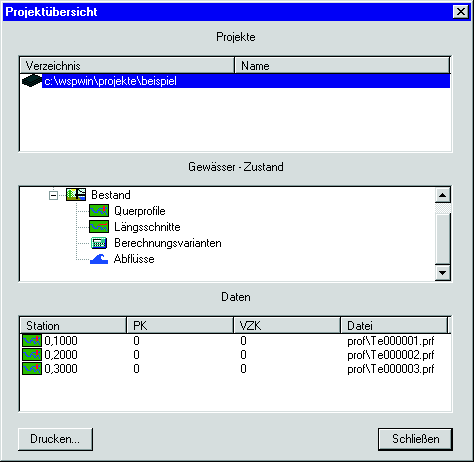
\includegraphics[width=0.8\textwidth]{Projektuebersicht}
   \caption{Dialogfenster \dialog{Projekt\"{u}bersicht}}
   \label{Fortgeschrittene Abb Projektuebersicht}
\end{figure}

In dem mittleren Fenster werden die einzelnen Komponenten des ausgew\"{a}hlten Projektes dargestellt. Ausgehend von
Gew\"{a}ssernamen sind dies zun\"{a}chst die einzelnen Zu\-st\"{a}n\-de des Gew\"{a}ssers. Innerhalb der Zust\"{a}nde sind die zugeh\"{o}rigen
Querprofile, L\"{a}ngsschnitte, Berechnungsvarianten und Abfl\"{u}sse aufgelistet. Das untere Fenster zeigt die vorhandenen Daten
(Profildateien, L\"{a}ngsschnittdateien, Berechnungsvariantendateien und Abflu{\ss}dateien).


\subsection{Projekte kopieren}

\"{U}ber die Men\"{u}folge \menu{\marrow \underline{P}rojekt \marrow Projekt \underline{s}peichern unter} haben Sie die
M\"{o}glichkeit, da{\ss} gerade ge\"{o}ffnete Projekt in ein anderes Verzeichnis zu kopieren, um dort z.B. zu Testzwecken
Einstellungen zu modifizieren. Es erscheint ein Dialog, der Sie zur Eingabe des neuen Projektverzeichnisses auffordert.
Wenn das angegebene Verzeichnis noch nicht existiert, wird es automatisch neu angelegt. \"{U}ber den Schalter
\schalter{Suchen...} haben Sie aus der Standard-Windows-Maske heraus auch die M\"{o}glichkeit, einen Pfad zu suchen, der dann
im Editierfeld \feld{Verzeichnis} angezeigt wird und hier oder in dem Dialog \dialog{Projekt speichern unter} erg\"{a}nzt
werden kann.


\subsection{Projekte archivieren}

Projekte, die momentan nicht mehr gebraucht werden, k\"{o}nnen \"{u}ber \wspwin{} archiviert werden. W\"{a}hlen Sie hierzu die
Men\"{u}folge \menu{\marrow \underline{P}rojekt \marrow \underline{A}rchivieren \marrow archivieren} und selektieren Sie
anschlie{\ss}end das zu archivierende Projekt. Sie werden aufgefordert, da{\ss} Verzeichnis einzugeben, in dem Sie Ihr Projekt
archivieren m\"{o}chten. Sie k\"{o}nnen in diesem Arbeitsschritt einen neuen Namen f\"{u}r Ihr Verzeichnis vergeben und auch mehrere
Unterverzeichnisse anlegen. Das entsprechende Projekt wird anschlie{\ss}end aus der Projekt\"{u}bersichtsliste entfernt.

Mittels \menu{\marrow \underline{P}rojekt \marrow \underline{A}rchivieren \marrow zur\"{u}ckladen} kann es jederzeit wieder
aufgenommen werden. Eine Liste der archivierten Projekte befindet sich in der Datei \datei{wspwin.arh}, die sich im
Verzeichnis der Datei \datei{wspwin.prj} befindet und nicht ver\"{a}ndert werden sollte. Die Projektarchivierung beinhaltet
keine Datenkomprimierung.


\subsection{Projekte importieren}

\"{U}ber den Men\"{u}punkt \menu{\marrow \underline{P}rojekt \marrow \underline{I}mportieren \marrow Projekt
auf\underline{n}ehmen} k\"{o}nnen Projekte, die nicht im Projektvereichnis aufgelistet sind, importiert werden. Dies macht
beispielsweise Sinn, wenn sie Projektdaten von anderen Anwendern geschickt bekommen und weiterverarbeiten m\"{o}chten. Im
gleichen Men\"{u}punkt finden Sie auch das Untermen\"{u} \menu{ \marrow Projekteintrag \underline{l}\"{o}schen}. Im Gegensatz zu der
Funktion \schalter{L\"{o}schen} aus der Projektauswahlmaske heraus wird hier nur der Projekteintrag entfernt, das Verzeichnis
mit seinen Daten bleibt bestehen.


\subsection{Fremddaten}

\subsubsection{HYDRA-WSP}
\wspwin{} erm\"{o}glicht Ihnen die Konvertierung von bereits existierenden \"{a}lteren Datens\"{a}t\-zen im Format von HYDRAWSP
(LWA-Format) in ein Format, das von \wspwin{} sowohl rechnerisch wie auch grafisch verarbeitet werden kann.

Nach Aufruf des Men\"{u}punktes \menu{ \marrow \underline{P}rojekt \marrow \underline{F}remddaten  \marrow
\underline{H}YDRAWSP} erscheint ein Dialogfenster, das Sie zur Auswahl einer oder mehrerer zu konvertierender Dateien
auffordert.  Die Dateien m\"{u}ssen \"{u}ber die Endung \datei{*.wsp} verf\"{u}gen (ggf. umbenennen). Die konvertierten Dateien werden
alle in ihrem aktuellen Projekt abgelegt, das Ihnen in einer Sicherheitsabfrage nochmals angezeigt wird.

F\"{u}r jede konvertierte Datei wird eine neue Vernetzungsdatei eingerichtet. Dazu sind jeweils die Schl\"{u}sseldaten
Gew\"{a}ssername, Datum und Zustand von Ihnen zu definieren. Hierbei erscheint zun\"{a}chst noch einmal der Name der zu
konvertierenden Datei, den Sie mit \schalter{OK} best\"{a}tigen, gefolgt von dem bekannten Dialogfenster zur Definition der
Schl\"{u}sseldaten. Dieser Vorgang wird so oft wiederholt, wie Sie zu konvertierende Dateien ausgew\"{a}hlt haben. Nach der
letzten Datei wird schlie{\ss}lich ein Konvertierungsprogramm gestartet, das die neuen Vernetzungs- und Profildateien f\"{u}r Sie
anlegt. Die Dateien k\"{o}nnen dann wie gewohnt von Ihnen weiter bearbeitet werden. Auch die Steuerdaten f\"{u}r die Berechnung
werden \"{u}bernommen. Beachten Sie aber, da{\ss} jeweils nur der erste Abflu{\ss}zustand in das \wspwin{}-Format \"{u}berf\"{u}hrt wird.

Nach Abschlu{\ss} der Konvertierung wird eine Meldung ausgegeben. Meldungen \"{u}ber aufgetretene Fehler k\"{o}nnen in der Datei
\datei{\mbox{error.log}} eingesehen werden. Ein Protokoll der Umwandlung findet sich in der Datei \datei{lwa2b.log}.

\subsubsection{DA66}
\wspwin{} kann mit einem Zusatzmodul zur Konvertierung von Vermessungsdaten im Format DA66 ins \wspwin{}-Format geliefert
werden. Die Option ist dann unter dem Men\"{u}punkt \menu{ \marrow \underline{P}rojekt  \marrow \underline{F}remddaten \marrow
\underline{D}A66} verf\"{u}gbar. Nach diesem Aufruf werden Sie in einem Standard-Windows-Dialog zur Auswahl der DA66-Datei
aufgefordert. Sobald Sie die Datei ausgew\"{a}hlt haben, m\"{u}ssen Sie die Schl\"{u}sseldaten f\"{u}r eine neue Vernetzungsdatei angeben.
Im Anschlu{\ss} daran wird die Datei konvertiert.

\begin{figure}[hbt]
   \centering
   \input{Fortgeschrittene/tab/FormatDA66.tab}
   \caption{Ausschnitt aus einer Datei im DA66-Format}
   \label{Fortgeschrittene Abb FormatDA66}
\end{figure}

Nach erfolgreicher Umwandlung erhalten Sie eine Meldung \"{u}ber die Anzahl angelegter Profile. Wenn Sie nun Ihre neu
angelegte Zustandsdatei \"{o}ffnen, sind hier ihre neuen Profile noch nicht eingetragen. Sie m\"{u}ssen die konvertierten
Profildateien \"{u}ber die Schaltfl\"{a}che \schalter{Profile aufnehmen} aus der Maske zur \dialog{Erfassung/Editierung der
Zustandsdatei} heraus in den Zustand eingliedern. Die neuen Profildateien sind im Unterverzeichnis \datei{\textbackslash
prof} Ihres aktuellen Projektes abgelegt. Ihre Endung lautet nicht wie gewohnt \datei{*.prf}, sondern zur leichteren
Identifikation \datei{*.dat}. Sie brauchen die Profile beim Aufnehmen nicht zu kopieren.

\subsubsection{Waspila}
Unter \menu{ \marrow Fremddaten \marrow WSPWIN $\rightarrow$ Waspila} im Men� \menu{\marrow Projekt} haben Sie die M�glichkeit Daten, die im Format des Programms WASPILA abgelegt wurden, in \wspwin{} zu importieren. Sie werden zun�chst dazu aufgefordert, die Start-Datei auszuw�hlen, in der das Arbeitsverzeichnis (z.B. \datei{C:/projekt/}), sowie die Dateinamen der Dateien hinterlegt sind, die die Profilgeometrie, die Rauheiten und sonstige Charakteristika enthalten. 

\begin{figure}[hbt]
   \centering
   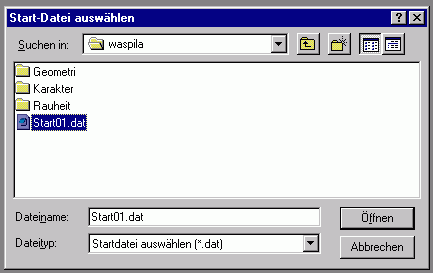
\includegraphics[width=0.8\textwidth]{waspila}
   \caption{Auswahl der Startdatei aus einem WASPILA-Projekt}
   \label{Fortgeschrittene Abb Waspila}
\end{figure}

Ausgehend von dieser Start-Datei werden in den Unterverzeichnissen GEOMETRI, KARAKTER und RAUHEIT die entsprechenden Dateien eingelesen. Der Benutzer wird dazu aufgefordert, Gew�ssername und Zustandsbezeichnung f�r eine neu anzulegende Zustandsdatei anzugeben. Sodann werden automatisch eine Zustandsdatei, sowie die Profile mit den entsprechenden Datens�tzen angelegt.

\subsubsection{Jabron}
Profildaten, die mit \wspwin{} im BCE-Format erstellt wurden, k\"{o}nnen \"{u}ber die Schnittstelle \menu{ \marrow
\underline{F}remddaten \marrow \underline{W}SPWIN--$>$JABRON} im Men\"{u} \menu{ \marrow \underline{P}rojekt} ins Datenformat
des Programms JABRON umgewandelt werden. Die Umwandlung erfolgt immer f\"{u}r eine komplette Zustandsdatei, die Sie aus Ihrem
aktuellen Projekt ausw\"{a}hlen.

Die konvertierten Daten werden im Unterverzeichnis \datei{\textbackslash prof} Ihres ge\"{o}ffneten Projektes unter dem Namen
\datei{jabron.pro} abgespeichert. Die Datei wird bei wiederholtem Aufruf des Konvertierungsprogramms stets \"{u}berschrieben.
Konvertiert werden die Datens\"{a}tze \afz{Gel\"{a}ndeh\"{o}he}, \afz{Rauheit} (unabh\"{a}ngig davon, ob es sich um $k_S$- oder
$k_{ST}$-Werte handelt), \afz{Trennfl\"{a}chen} und \afz{Durchstr\"{o}mte Bereiche}. Ebenso k\"{o}nnen Dateien im Format von JABRON
ins \wspwin{}-Format konvertiert werden.


\subsubsection{CADDY}
\wspwin{} bietet die M\"{o}glichkeit, Profilgeometrien aus dem Vermessungsprogramm CADDY zu \"{u}bernehmen. Der Import der
\datei{*.que}-Dateien erfolgt \"{u}ber den Men\"{u}punkt \menu{\marrow \underline{F}remd\-da\-ten \marrow \underline{C}ADDY}. Es
k\"{o}nnen mehrere Profile gleichzeitig in ein existierendes Projekt aufgenommen werden. Daf\"{u}r sind lediglich Zustand und
Gew\"{a}ssername anzugeben.


\subsubsection{Access}
Sie haben die M�glichkeit in \wspwin Vermessungsdaten zu importieren, die in einer ACCESS-Datenbank abgelegt wurden. Die Daten m�ssen hierzu aus ACCESS heraus als TXT-Datei exportiert werden und in folgendem Format vorliegen.

\begin{verbatim}
Datei STATION.TXT:
NR	; STATION;	GEW�SSERNAME

176,00;"53+173";"Gr. Hase"
177,00;"53+257";"Gr. Hase"
178,00;"53+332";"Gr. Hase"
179,00;"53+424";"Gr. Hase"
180,00;"53+518";"Gr. Hase"
181,00;"53+563";"Gr. Hase"
182,00;"53+611";"Gr. Hase"
183,00;"53+656";"Gr. Hase"
184,00;"53+701";"Gr. Hase"
185,00;"53+736";"Gr. Hase"
186,00;"53+807";"Gr. Hase"
187,00;"53+864";"Gr. Hase"
1,00;"00+174";"Fladderkanal"
2,00;"00+328";"Fladderkanal"
3,00;"00+530";"Fladderkanal"
4,00;"00+625";"Fladderkanal"
5,00;"00+839";"Fladderkanal"
6,00;"01+109";"Fladderkanal"
7,00;"01+369";"Fladderkanal"
8,00;"01+599";"Fladderkanal"
9,00;"01+822";"Fladderkanal"
10,00;"01+982";"Fladderkanal"
11,00;"02+063";"Fladderkanal"
\end{verbatim}

\begin{verbatim}
Datei: PROFILE.TXT
NR;	Z-Wert;	Rechtswert;	Hochwert;

1,00;24,01;3433992,90;5841859,90
1,00;23,96;3433991,30;5841862,10
1,00;24,09;3433990,50;5841863,10
1,00;23,93;3433989,40;5841864,80
1,00;23,63;3433988,40;5841865,90
1,00;22,73;3433986,90;5841868,30
1,00;22,15;3433985,50;5841870,10
1,00;21,91;3433984,80;5841871,10
1,00;21,13;3433984,40;5841871,70
1,00;20,65;3433984,10;5841872,40
2,00;24,41;3434123,70;5841941,00
2,00;24,41;3434121,60;5841944,20
2,00;24,46;3434120,30;5841946,30
2,00;24,33;3434118,60;5841948,90
2,00;24,27;3434117,60;5841950,30
\end{verbatim}

Die Daten sind wie folgt zu importieren.
W�hlen Sie aus einem ge�ffneten Projekt heraus die Men�folge: PROJEKT- FREMDDATEN- ACCESS. W�hlen Sie anschlie�end den Pfad, in dem sich die PROFILE.txt-Datei befindet und unmittelbar danach das Verzeichnis f�r Ihre STATIONEN.txt-Datei. Unter Dateiname erscheint jeweils PROFILE oder STATIONEN. Es wird f�r jedes Gew�sser eine separate Zustandsdatei angelegt, in die die Profile konvertiert werden.

\begin{figure}[hbt]
   \centering
   \includegraphics[width=0.8\textwidth]{access}
   \caption{Vermessungsdaten in einer ACCESS-Datenbank}
   \label{Fortgeschrittene Abb ACCESS Daten}
\end{figure}

\begin{figure}[hbt]
   \centering
   \includegraphics[width=0.8\textwidth]{access2}
   \caption{W�hlen der Stationen-Datei}
   \label{Fortgeschrittene Abb ACCESS Datei}
\end{figure}


\clearpage
%%%%%%%%%%%%%%%%%%%%%%%%%%%%%%%%%%%%%%%%%%%%%%%%%%%%%%%%%%%%%%%%%%%%%%%%%%%%%%%%%%%%%%%%%%%%%%%%%%%%%%%%%%%%%%%%%%%%%%%%%%%%
\section{Zust\"{a}nde bearbeiten}
%%%%%%%%%%%%%%%%%%%%%%%%%%%%%%%%%%%%%%%%%%%%%%%%%%%%%%%%%%%%%%%%%%%%%%%%%%%%%%%%%%%%%%%%%%%%%%%%%%%%%%%%%%%%%%%%%%%%%%%%%%%%

\subsection{Zust\"{a}nde kopieren}

Wenn Sie eine neue Vernetzungsdatei anlegen und einen Gew\"{a}ssernamen angeben, f\"{u}r den bereits eine Zustandsdatei existiert,
erscheint ein neuer Dialog, der Ihnen s\"{a}mtliche im Projekt vorhandenen Profildateien dieses Gew\"{a}ssers auflistet. Sie
k\"{o}nnen diese dann markieren und mit \schalter{OK} dem neuen Zustand zuordnen. Dies ist z.B. dann von Vorteil, wenn Sie
einen Istzustand und einen Planungsfall bearbeiten und bei letzterem streckenweise Profile nicht ver\"{a}ndert werden. Im
Gegensatz zu der Option \schalter{Profile aufnehmen} aus der Dialogmaske \dialog{Erfassung/Editierung der Zustandsdatei}
k\"{o}nnen hier Profile anhand ihrer Schl\"{u}sseldaten ausgew\"{a}hlt werden.

Sollten Sie keine Profile aufnehmen m\"{o}chten, so w\"{a}hlen Sie die Schaltfl\"{a}che \schalter{Abbruch}. Die Anzahl der auf diese
Weise aufnehmbaren Profile ist auf $25$ begrenzt. Sollen weitere Profile aufgenommen werden, hat dies \"{u}ber die Option
\afz{Profile aufnehmen} aus der Maske \dialog{Erfassung/Editierung der Zustandsdatei} heraus zu erfolgen (siehe
Abschnitt~\ref{Einstieg Subsec ProfilAnlegen}).

Besteht der zu kopierende Zustand aus mehr als 25~Profildateien und sind f\"{u}r den neuen Zustand nur geringe \"{A}nderungen an
den Profilen erforderlich, so kann es von Vorteil sein, zun\"{a}chst den gesamten Zustand zu kopieren. Dies geschieht mit
Hilfe des Men\"{u}s \menu{ \marrow Z\underline{u}stand \marrow Zu\underline{s}tand speichern unter}. Es erscheint die in
Abschnitt~\ref{Einstieg Subsec ProfilAnlegen} beschriebene Maske \dialog{neue Vernetzungsdatei anlegen}, in die sie den
Gew\"{a}ssernamen und den Namen des neuen Zustands eintragen m\"{u}ssen. Kopiert werden unter neuen Dateinamen alle Profile, die
Abflu{\ss}- und Verlustdatei sowie die Berechnungsvarianten.
\begin{hinweis}
   Beachten Sie, da{\ss} beim Aufnehmen von Profilen ohne Kopieren (d.h. lediglich Erstellen eines Verweises) die
   Profildateien in den beiden Zust\"{a}nden identisch sind. \"{A}nderungen am Profil im Planungsfall haben beispielsweise daher
   auch \"{A}nderungen im Istzustand zur Folge.
\end{hinweis}


\subsubsection{Beispiel - Zust�nde kopieren}

Legen Sie eine zweite Zustandsdatei f\"{u}r das Beispielgew\"{a}sser \afz{Testbach} an. Geben Sie als Gew\"{a}ssernamen \afz{Testbach}
und als Zustand \afz{Planung} an. Dazu w\"{a}hlen Sie zun\"{a}chst aus dem Dialog \dialog{Auswahl der Zustandsdatei} die
Schaltfl\"{a}che \schalter{Neue Zustandsdatei}. In den nun folgenden Dialog geben Sie ein:
\begin{quote}
   \begin{tabular}{ll}
      Gew\"{a}ssername:  &  \beisp{Testbach} \\
      Zustand:       &  \beisp{Planung}
   \end{tabular}
\end{quote}
Nach der Best\"{a}tigung der Eingabe mit \schalter{OK} \"{o}ffnet sich der Dialog, mit dessen Hilfe Sie Profildateien in den neuen
Zustand \"{u}bernehmen k\"{o}nnen. W\"{a}hlen Sie hier die erste und dritte Profildatei aus und best\"{a}tigen Sie mit \schalter{OK}. Nur
das Profil an Station $0,2~\unit{km}$ soll baulich ver\"{a}ndert werden und wird daher sp\"{a}ter kopiert oder neu erstellt.


\subsection{Strangtabelle}

Standardm\"{a}{\ss}ig wird die Strangtabelle mit einer sortierten Liste der Stationswerte aus s\"{a}mtlichen zum Zustand geh\"{o}rigen
Profilen vorbesetzt und zwar sowohl beim Neuanlegen, wie auch beim Aufnehmen oder Konvertieren von Profilen. Die
Profilabst\"{a}nde werden aus diesen Stationswerten zun\"{a}chst f\"{u}r die Vorl\"{a}nder und den Flu{\ss}schlauch einheitlich besetzt. Die
Stationwerte nehmen dabei von der M\"{u}ndung zur Quelle hin zu. \"{U}ber die Editierfelder der Strangtabelle wird die M\"{o}glichkeit
geboten, die vorgegebenen Werte zu \"{a}ndern. So k\"{o}nnen z.B. unterschiedliche Abst\"{a}nde zwischen den Profilen f\"{u}r Vorl\"{a}nder
und Flu{\ss}schlauch (z.B. bei stark m\"{a}andrierenden Gew\"{a}ssern) eingegeben werden. Die eingegebenen Werte werden auf
Plausibilit\"{a}t gepr\"{u}ft.

Die Auswahl der Profile in der Strangtabelle ist entscheidend f\"{u}r die sp\"{a}tere Wasserspiegellagenberechnung, die nur
Profile ber\"{u}cksichtigt, die durch eine Strangtabelle verkn\"{u}pft wurden. Die Strangtabelle besteht aus mehreren
Gew\"{a}sserstr\"{a}ngen, d.h. jeweils aus einem Anfangs- und einem Endprofil, wobei das Endprofil des vorherigen Stranges
zugleich das Anfangsprofil des nachfolgenden Gerinneabschnittes darstellt. Beim Eingeben der Steuerdaten f\"{u}r die
Wasserspiegellagenberechnung k\"{o}nnen hieraus eine Anfangs- und Endstation f\"{u}r die Berechnung ausgew\"{a}hlt werden. Wenn die
Strangtabelle ge\"{a}ndert wird, aber bereits Randbedingungen (Abflu{\ss}- oder Verlustdatei) und Berechnungsvarianten existieren,
werden die betroffenen Werte gel\"{o}scht.

Bei verzweigten Gerinneabschnitten und bei mehrgliedrigen Profilen kann die Strangtabelle nicht mehr automatisch
vorbesetzt werden. In diesem Fall erh\"{a}lt der Benutzer die M\"{o}glichkeit selbst festzulegen, an welcher Position der
Strangtabelle ein neues Profil einzuf\"{u}gen ist (siehe Abschnitte~\ref{Sonderprofile Subsec Mehrfeldbruecken} und
\ref{Sonderprofile Sec VerzweigteSysteme}). Beachten Sie bitte, da{\ss} beim automatischen Vorbesetzen der Strangtabelle die
Profilabst\"{a}nde aus der Differenz der Stationsangaben errechnet werden. Bei verzweigten Systemen oder starker Kr\"{u}mmung des
Flu{\ss}laufs kann daher eine Korrektur der Werte bez\"{u}glich der Profilabst\"{a}nde erforderlich sein.


\subsection{Der Umgang mit der Rauheits- und Bewuchsdatenbank}
\label{Fortgeschrittene Subsec Rauheitsdatenbank}

In \wspwin{} steht Ihnen im Grafikeditor bzw. alphanumerischen Editor f\"{u}r die Datens\"{a}tze \afz{Rauheit ks}, \afz{Rauheit
KST}, \afz{Bewuchsabst. AX in Flie{\ss}r.}, \afz{Bewuchsabst. AY quer Flie{\ss}r.}, \afz{Bewuchsdurchmesser DP} die M\"{o}glichkeit
zur Verf\"{u}gung, eine Datenbank anzulegen. Dies ist nach Wahl des entsprechenden Datensatzes \"{u}ber die Schaltfl\"{a}che
\schalter{Datenbank} im Dialogfenster \dialog{Bereiche editieren} m\"{o}glich. Die drei Datenbanken werden im Startverzeichnis
von \wspwin{} gespeichert und sind somit aus jedem Projekt heraus verf\"{u}gbar.
\begin{figure}
   \centering
   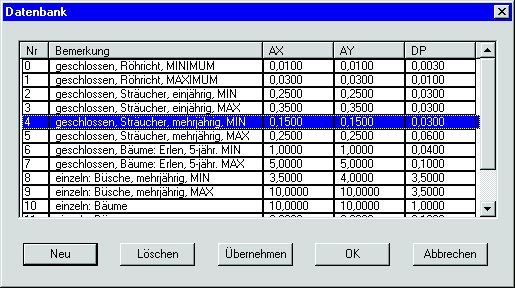
\includegraphics[width=0.9\textwidth]{DialogDatenbank}
   \caption{Bewuchsdatenbank}
   \label{Fortgeschrittene Abb Datenbank}
\end{figure}

Sollen neue Werte in die Datenbank aufgenommen werden, ist die Option \schalter{Neu} zu w\"{a}hlen. Daraufhin erhalten Sie
eine neue Zeile. Geben Sie einen Text f\"{u}r Bemerkung (maximal 40~Zeichen) ein und wechseln Sie dann per Tabulatortaste oder
Maus auf das Feld f\"{u}r die zugeh\"{o}rigen Werte.

Datenbankeintr\"{a}ge k\"{o}nnen durch Selektion des entsprechenden Listeneintrages und Bet\"{a}tigen der Schaltfl\"{a}che
\schalter{L\"{o}schen} jederzeit wieder aus der Datenbank entfernt werden. Ebenso kann der Eintrag durch Markieren und
\"{U}berschreiben der Editierfelder ge\-\"{a}n\-dert werden. Die Eintragungen werden beim Verlassen der Datenbank mit
\schalter{OK} gespeichert. \schalter{Abbruch} bewirkt ein Verlassen der Datenbank ohne Speicherung der vorgenommenen
\"{A}nderungen.

Neben dem Anlegen der Rauheitsdatenbank haben Sie auch die M\"{o}glichkeit, Werte aus der Datenbank auszuw\"{a}hlen und \"{u}ber die
Schaltfl\"{a}che \schalter{\"{U}bernehmen} direkt in eine Profildatei zu \"{u}bertragen. Nachdem Sie \schalter{\"{U}bernehmen} gew\"{a}hlt
haben, erscheint wieder die Dialogmaske \dialog{Bereiche editieren} zur Angabe des Anfangs- und Endprofilpunktes, sowie
eines Offset-, Faktor- oder neuen Wertes. Im Falle einer \"{U}bernahme von Datens\"{a}tzen aus der Datenbank ist der entsprechende
neue Wert schon eingetragen, so da{\ss} der Benutzer nur noch den Bereich einzugeben und mit \schalter{OK} zu best\"{a}tigen hat.
Bei der \"{U}bernahme von Bewuchsparametern erfolgt zus\"{a}tzlich eine Abfrage, ob alle drei Bewuchsparameter \"{u}bernommen werden
sollen. Sollte dies nicht gew\"{u}nscht sein, kann auch nur ein einzelner Parameter als aktueller Datensatz im Grafik-Editor
gew\"{a}hlt und die Frage mit \schalter{Nein} beantwortet werden. Beachten Sie, da{\ss} bei der Bewuchsdatenbank zur \"{U}bernahme von
Datens\"{a}tzen in die Profildatei die Datenblocktypen bereits angelegt sein m\"{u}ssen.




\subsection{Rauheiten global \"{a}ndern}

Die Rauheiten der einzelnen Profile k\"{o}nnen direkt im grafischen bzw. alphanumerischen Editor den einzelnen Profilen
zugeordnet werden. \wspwin{} bietet dar\"{u}ber hinaus jedoch auch noch die M\"{o}glichkeit, die Rauheiten in mehreren Profilen
gleichzeitig zu \"{a}ndern. Bedingung daf\"{u}r ist jedoch, da{\ss} der Datensatz \afz{Rauheit} bereits in den Profilen vorhanden ist.

Mit Hilfe des Men\"{u}punktes \menu{ \marrow Z\underline{u}stand \marrow \underline{R}auheiten \"{a}ndern} gelangen Sie in einen
Dialog (Abbildung~\ref{Fortgeschrittene Abb DialogRauheitenAendern}), in dem sie jedem Profil eine neue Rauheit f\"{u}r das
linkes Vorland, den Flu{\ss}schlauch und das rechte Vorland zuweisen k\"{o}nnen.
\begin{figure}
   \centering
   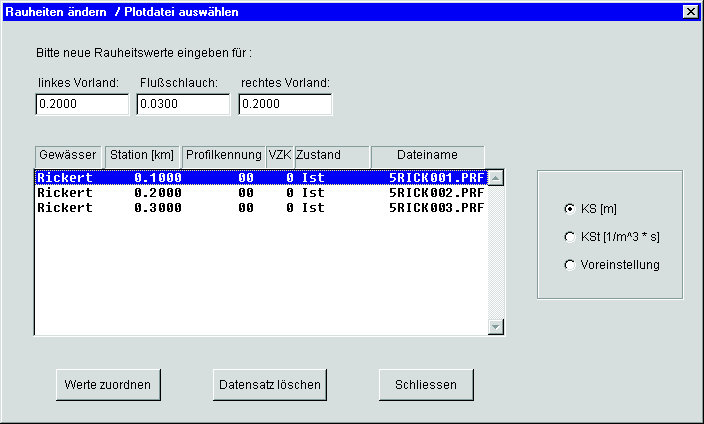
\includegraphics[width=1.0\textwidth]{DialogRauheitenAendern}
   \caption{Dialogfenster Rauheiten \"{a}ndern}
   \label{Fortgeschrittene Abb DialogRauheitenAendern}
\end{figure}
Durch Festhalten der \schalter{Strg}-Taste k\"{o}nnen mehrere Profile gleichzeitig mit der Maus ausgew\"{a}hlt werden. Die Eingabe
der neuen Rauheiten erfolgt in die daf\"{u}r vorgesehenen Felder oberhalb der Profilauswahltabelle. \"{U}ber die Schaltfl\"{a}che
\schalter{Werte zuordnen} werden die neuen Rauheiten in die Profildateien \"{u}bernommen. Es erfolgt eine Abfrage, ob sie
weitere Profile bearbeiten m\"{o}chten. Sie k\"{o}nnen auch das Protokoll zur Bearbeitung der Profildateien einsehen.

Die Schaltfl\"{a}che \schalter{Datensatz l\"{o}schen} hat die gleiche Funktion wie im alphanumerischen und im grafischen Editor.
Der Datensatz \afz{Rauheit} kann hier in den ausgew\"{a}hlten Profilen komplett gel\"{o}scht werden. Das Auswahlfeld auf der
rechten Seite erlaubt Ihnen einen anderen Rauheitsdatensatz auszuw\"{a}hlen.



\subsection{Die Eingabe von Einzelverlusten}
\label{Fortgeschrittene Subsec Einzelverluste}

Der Ber\"{u}cksichtigung von Str\"{o}mungsverlusten kommt bei der Berechnung von Wasserspiegellagen eine erhebliche Bedeutung zu.
Prinzipiell wird zwischen kontinuierlich zunehmenden (Wandreibungsverlust) und \"{o}rtlich konzentrierten Verlusten
unterschieden. Der Wandreibungsverlust wird \"{u}ber entsprechende Reibungsans\"{a}tze im Flie{\ss}gesetz be\-r\"{u}ck\-sichtigt. Die
Einzelverluste lassen sich durch den allgemeinen Verlustansatz in der Hydraulik erfassen:
\begin{equation}
   H_{ZV} = \zeta \cdot \frac{v_{i-1}^2}{2g}
      \label{Fortgeschrittene Gl Einzelverluste}
\end{equation}
Der Verlustbeiwert $\zeta$ ist abh\"{a}ngig von der Art und der Form der St\"{o}rstelle.

\subsubsection{Ber\"{u}cksichtigung der Erweiterungsverluste nach dem Ansatz von \autor{Borda-Carnot}}
Die Verlusth\"{o}he infolge einer Aufweitung des Querschnitts kann nach \autor{Borda-Carnot} wie folgt bestimmt werden:
\begin{equation}
   H_{ZV} = c_i \cdot \frac{(v_i - v_{i-1})^2}{2g}
      \label{Fortgeschrittene Gl VerlustBordaCarnot}
\end{equation}
Dabei stellen $v_i$ und $v_{i-1}$ jeweils die mittleren Geschwindigkeiten im Gesamtquerschnitt dar. Der Faktor $c_i$ ist
ein frei zu w\"{a}hlender Abminderungsfaktor.

\subsubsection{Verengungsverluste}
Der Verlustbeiwert bei Verengungen kann f\"{u}r Kompaktquerschnitte in erster N\"{a}herung aus dem Fl\"{a}chenverh\"{a}ltnis abgesch\"{a}tzt
werden:
\begin{equation}
   \zeta_E = c_i \cdot \left(\frac{A_{i-1}}{A_i} - 1 \right)^2
      \label{Fortgeschrittene Gl Verengungsverluste}
\end{equation}
Die Verlusth\"{o}he erh\"{a}lt man dann mit Hilfe von Gleichung~\ref{Fortgeschrittene Gl Einzelverluste}.

\subsubsection{Dateneingabe in der Verlustdatei}
Die Verlustbeiwerte werden (wie auch die Abflu{\ss}daten) in einer separaten Verlustdatei gespeichert. \"{U}ber das Men\"{u}
\menu{\marrow Z\underline{u}stand \marrow Einzel\underline{v}erluste} \"{o}ffnen Sie den Dialog zur Eingabe der erforderlichen
Beiwerte.
\begin{figure}[hbt]
   \centering
   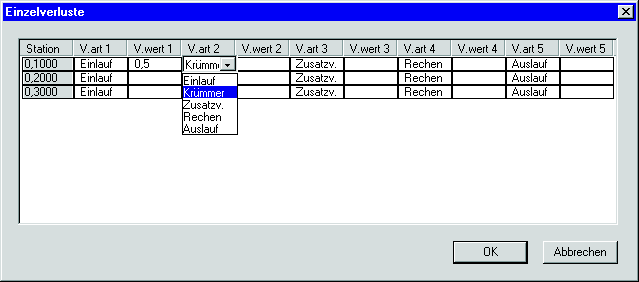
\includegraphics[width=1.0\textwidth]{Verlustdatei}
      \caption{Dialogfenster zur Eingabe der Parameter in die Verlustdatei}
      \label{Fortgeschrittene Abb Verlustdatei}
\end{figure}

An jeder Station k\"{o}nnen bis zu f\"{u}nf verschiedene Beiwerte eingegeben werden. Neben jedem Wertefeld finden Sie eine Liste
aus der sie die entsprechende Verlustart ausw\"{a}hlen k\"{o}nnen. Die Eingabe der Verlustart hat keinen Einflu{\ss} auf die
Berechnung, Sie dient lediglich Ihrer Information.

Die Interpretation der eingegebenen Werte vom Programm ist abh\"{a}ngig von den Festlegungen bei der Eingabe der
Steuerparameter f\"{u}r die Berechnung. Weitere Informationen hierzu finden Sie in Abschnitt~\ref{Fortgeschrittene Subsec
Einstellungen} dieses Handbuchs.

Prinzipiell sind die \"{o}rtlichen Verlustbeiwerte $\zeta$ jeweils im oberstromigen Profil einzugeben. Dies gilt auch f\"{u}r
Verluste an Verengungen im Br\"{u}ckenbereich. Soll der Verengungsverlust nach Gleichung~\ref{Fortgeschrittene Gl
Verengungsverluste} automatisch berechnet werden, so ist dies durch die Eingabe eines negativen Wertes an der betreffenden
Station zu kennzeichen. Der negative Wert wird dann bei entsprechender Vereinbarung in den Steuerdaten der Berechnung als
Abminderungsfaktor $c_i$ interpretiert. Die Eingabe eines positiven Wertes kann in Abh\"{a}ngigkeit von den in
Abschnitt~\ref{Fortgeschrittene Subsec Einstellungen} zu treffenden Vereinbarungen f\"{u}r die Berechnung sowohl als \"{o}rtlicher
Verlustbeiwert $\zeta$ nach Gleichung~\ref{Fortgeschrittene Gl Einzelverluste} (keine automatische Berechnung von
Einzelverlusten) als auch als Abminderungsfaktor $c_i$ f\"{u}r die automatische Ber\"{u}cksichtigung der Erweiterungsverluste nach
Gleichung~\ref{Fortgeschrittene Gl VerlustBordaCarnot} gedeutet werden.



\subsection{Vergleich von Zust\"{a}nden und Profilen}
\label{Fortgeschrittene Subsec Vergleichszustaende}

Sie k\"{o}nnen mit Hilfe von \wspwin{} Vergleiche zwischen einzelnen Zust\"{a}nden hinsichtlich Fl\"{a}chen- und Massenberechnung
vornehmen. Voraussetzung daf\"{u}r ist, da{\ss} bei den zu vergleichenden Profilen neben dem Gew\"{a}ssernamen und der Station auch
jeweils erste und letzte Profilpunkt (Gel\"{a}ndekoordinaten) \"{u}bereinstimmt.

\subsubsection{Vergleich der Gel\"{a}ndekontur}
Ihr aktueller Zustand bildet f\"{u}r den Vergleich den Referenzzustand. F\"{u}r den Vergleich des kompletten Zustandes mu{\ss} die
Dialogmaske \dialog{Erfassung/Editierung der Zustandsdatei} ge\"{o}ffnet sein. \"{U}ber das Men\"{u} \menu{\marrow Z\underline{u}stand
\marrow Ver\underline{g}leichszutand \marrow \underline{G}el\"{a}nde \marrow \underline{n}eu} k\"{o}nnen sie Ihren
Vergleichszustand ausw\"{a}hlen. In den Profildateien Ihres Referenzzustandes wird nun der Datensatz \afz{2. Gel\"{a}nde H\"{o}he} mit
den Gel\"{a}ndedaten aus dem Vergleichszustand angelegt.

Bei der Auswahl des Datensatzes im Grafikeditor werden nun sowohl die Gel\"{a}ndekontur des Referenzzustandes, als auch die
Gel\"{a}ndekontur des Vergleichszustandes angezeigt. Der Datensatz \afz{2.Gel\"{a}nde H\"{o}he} kann \"{u}ber das Untermen\"{u} \menu{\marrow
\underline{G}el\"{a}nde \marrow \underline{l}\"{o}schen} wieder aus allen Profilen des Referenzzustandes entfernt werden.

\subsubsection{Fl\"{a}chenberechnung}
Neben dem reinen Verkn\"{u}pfen der Profile aus zwei geometrischen Zust\"{a}nden (d.h. der parallelen Darstellung von zwei
Gel\"{a}ndeh\"{o}hen in den Profilen) kann auch eine Fl\"{a}chenberechnung des Auf- und Abtrags zwischen den Profilen zweier zu
vergleichender Zust\"{a}nde durchgef\"{u}hrt werden.

Die zustandsbezogene Fl\"{a}chenberechnung erfolgt analog der Gel\"{a}ndeverkn\"{u}pfung \"{u}ber die Men\"{u}folge \menu{\marrow
Z\underline{u}stand \marrow Ver\underline{g}leichszustand \marrow \underline{F}l\"{a}che \marrow \underline{n}eu}. F\"{u}r alle
Profile, deren Stationen im Referenz- und Vergleichszustand identisch sind und bei denen der erste und letzte Profilpunkt
\"{u}bereinstimmen, werden die Datens\"{a}tze \afz{2.Gel\"{a}nde H\"{o}he} und \afz{Fl\"{a}che} angelegt, nachdem \"{u}ber die bekannte
Dialogmaske ein Vergleichszustand ausgew\"{a}hlt wurde. Sollte bereits eine Gel\"{a}ndeverkn\"{u}pfung oder Fl\"{a}chenberechnung
existieren, erscheint zun\"{a}chst die Abfrage, ob die alte Verkn\"{u}pfung zu l\"{o}schen ist, oder ob die bereits existierende
Gel\"{a}ndeverkn\"{u}pfung der Fl\"{a}chenberechnung zugrundegelegt werden soll. Falls Sie sich unschl\"{u}ssig sind, k\"{o}nnen Sie den
Vorgang auch \"{u}ber die Option \schalter{Abbrechen} beenden.

Nachdem Sie eine Fl\"{a}chenberechnung erfolgreich durchgef\"{u}hrt haben, k\"{o}nnen Sie den berechneten Auf- und Abtrag f\"{u}r jedes
Profil im alphanumerischen bzw. grafischen Editor betrachten. Der Datensatz \afz{Fl\"{a}che} enth\"{a}lt die einzelnen
Fl\"{a}chenwerte. Diese beziehen sich jeweils auf den Bereich rechts vom zugeh\"{o}rigen $y$-Wert. Positive Werte charakterisieren
dabei Auftrags- und negative Abtragsfl\"{a}chen. Neben den Einzelwerten werden in einem zus\"{a}tzlichen Fenster jeweils die
Summen des Auf- und Abtragsfl\"{a}chen, sowie die Gesamtsumme der Fl\"{a}chendifferenz ausgegeben. Der in allen Profilen
eingef\"{u}gte Datensatz \afz{Fl\"{a}che} kann wiederum \"{u}ber das Untermen\"{u} \menu{ \marrow \underline{F}l\"{a}che \marrow
\underline{l}\"{o}schen} aus allen Profildateien des Referenzzustandes entfernt werden.

\subsubsection{Vergleich einzelner Profile}
In gleicher Weise wie der Vergleich der Gel\"{a}ndekontur und die Fl\"{a}chenberechnung f\"{u}r komplette Zust\"{a}nde erfolgen kann, ist
es auch m\"{o}glich nur einzelne Profildateien verschiedener Zust\"{a}nde zu vergleichen. Auch hier m\"{u}ssen Anfangs- und Endpunkt
der Gel\"{a}n\-dekoordinaten, sowie die Station und der Gew\"{a}ssername \"{u}bereinstimmen. Der Aufruf erfolgt hierbei \"{u}ber das Men\"{u}
\menu{ \marrow Z\underline{u}stand \marrow Ver\underline{g}leichszutand} aus dem grafischen oder alphanumerischen Editor
heraus. Die weitere Vorgehensweise entspricht dem Vergleich zweier kompletter Zust\"{a}nde.


\subsection{Profile verl\"{a}ngern}
\wspwin{} ist in der Lage, bereits existierende Profile mit weiteren Profilen zu verl\"{a}ngern, d.h. diese links oder rechts
an das aktuelle Profil anzuh\"{a}ngen. Die Option kann dann von Interesse sein, wenn Profile oder Vorl\"{a}nder nachvermessen
werden oder weitere Daten z.B. aus einem digitalen H\"{o}henmodell vorliegen, die an das bereits existierende Profil
angebunden werden sollen.

W\"{a}hlen Sie hierzu aus dem alphanumerischen oder grafischen Editor heraus die Option \schalter{Profil verl\"{a}ngern}. Sie
werden dazu aufgefordert eine Profildatei im \wspwin{}- oder BCE-Format (\datei{*.prf} / \datei{*.dat}) auszuw\"{a}hlen, mit
der ihre aktuelle gerade dargestellte Profildatei zu verl\"{a}ngern ist. Anschlie{\ss}end m\"{u}ssen Sie noch angeben, ob das
ausgew\"{a}hlte Profil links oder rechts angef\"{u}gt werden soll.


\subsection{Profile interpolieren}

Bei zu gro{\ss} gew\"{a}hlten Profilabst\"{a}nden, insbesondere bei einem Flie{\ss}wechsel, k\"{o}nnen Zwischenprofile erforderlich werden.
Daf\"{u}r bietet \wspwin{} die M\"{o}glichkeit der Profilinterpolation. In dem Men\"{u} \menu{\marrow Z\underline{u}stand} finden sie
den Unterpunkt \menu{ \marrow \underline{I}nterpolieren}.
\begin{figure}[hbt]
   \centering
   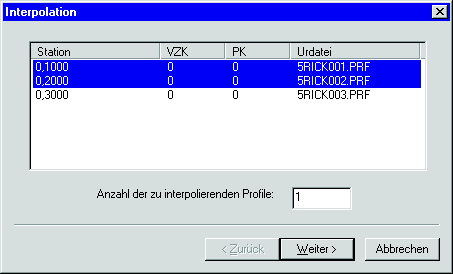
\includegraphics[width=0.8\textwidth]{Profilinterpolation1}
   \\[12pt]
   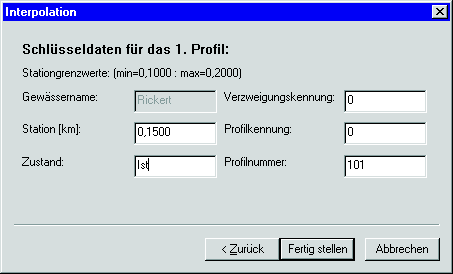
\includegraphics[width=0.8\textwidth]{Profilinterpolation2}
   \caption{Assistent zur Durchf\"{u}hrung von Profilinterpolationen}
   \label{Fortgeschrittene Abb Profilinterpolation}
\end{figure}

Mit seiner Hilfe gelangen sie in das Dialogfenster Abbildung~\ref{Fortgeschrittene Abb Profilinterpolation} oben. Hier
werden Sie zur Auswahl der Profile aufgefordert, zwischen denen interpoliert werden soll. Die Anzahl der einzuf\"{u}genden
Profile mu{\ss} in dem Feld \feld{Anzahl der zu interpolierenden Profile} eingegeben werden. Die Schaltfl\"{a}che
\schalter{Weiter} f\"{u}hrt sie in das nachfolgende Dialogfenster (Abbildung~\ref{Fortgeschrittene Abb Profilinterpolation},
unten), in dem Sie zur Festlegung der Schl\"{u}sseldaten entsprechend Abschnitt~\ref{Einstieg Subsec ProfilAnlegen} f\"{u}r das zu
interpolierende Profil aufgefordert werden. Entsprechend ihrer vorher gew\"{a}hlten Anzahl einzuf\"{u}gender Profile wiederholt
sich dieser Dialog. Die Profilinterpolation kann nicht bei Profilen mit R\"{u}ckspr\"{u}ngen (\autor{Gauss}-Profile) angewendet
werden.



\clearpage
%%%%%%%%%%%%%%%%%%%%%%%%%%%%%%%%%%%%%%%%%%%%%%%%%%%%%%%%%%%%%%%%%%%%%%%%%%%%%%%%%%%%%%%%%%%%%%%%%%%%%%%%%%%%%%%%%%%%%%%%%%%%
\section{Weitere Berechnungsoptionen}
%%%%%%%%%%%%%%%%%%%%%%%%%%%%%%%%%%%%%%%%%%%%%%%%%%%%%%%%%%%%%%%%%%%%%%%%%%%%%%%%%%%%%%%%%%%%%%%%%%%%%%%%%%%%%%%%%%%%%%%%%%%%

\subsection{Zus\"{a}tzliche Berechnungsm\"{o}glichkeiten}

\begin{figure}[hbt]
   \centering
   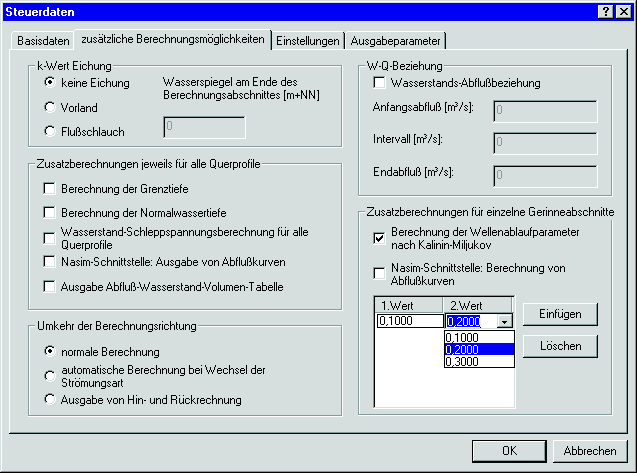
\includegraphics[width=1.0\textwidth]{ZusaetzlicheBerechnungsmoeglichkeiten}
   \caption{Registerkarte \dialog{Zus\"{a}tzliche Berechnungsm\"{o}glichkeiten}}
   \label{Fortgeschrittene Abb ZusaetzlicheBerechnungsmoeglichkeiten}
\end{figure}


\subsubsection{Eichung von Rauheitswerten}
Zur Bestimmung eines mittleren Rauheitsbeiwertes aus Me{\ss}werten (Kalibrierung) ist im Rechenprogramm folgendes
Verfahren~\cite{FelkelCanisius} zugrundegelegt:

Ausgehend von einer bekannten hydraulischen Randbedingung (Anfangswasserstand) wird die Wasserspiegellinie zun\"{a}chst mit
einem gesch\"{a}tzten Rauheitsbeiwert berechnet. Anschlie{\ss}end wird verglichen, ob der berechnete Endwasserspiegel mit dem
beobachteten \"{u}bereinstimmt. Ist dies nicht der Fall, so wird die Spiegellinienberechnung mit einem verbesserten
Rauheitsbeiwert wiederholt. Dieser Iterationsvorgang wird abgebrochen, wenn die Differenz zwischen vorgegebenem und
berechnetem Endwasserstand die gew\"{u}nschte Genauigkeitsschranke unterschreitet. Das Ergebnis ist ein mittlerer
Rauheitsbeiwert f\"{u}r den gew\"{a}hlten Abschnitt.

Im Falle gegliederter Querschnitte ist zun\"{a}chst der Rauheitsbeiwert des Flu{\ss}schlauchs f\"{u}r ein etwa bordvolles Hochwasser
zu bestimmen. Erst dann kann f\"{u}r ein ausuferndes Hochwasser der mittlere Rauheitsbeiwert der Vorlandfl\"{a}chen berechnet
werden.

Zur Eichung einer Flu{\ss}strecke kann jeder Flu{\ss}abschnitt gew\"{a}hlt werden, in dem \emph{kein} Flie{\ss}wechsel auftritt und in dem
gleichbleibende Rauheitsstrukturen vorliegen. F\"{u}r Strecken mit durchstr\"{o}mtem Bewuchs liegen noch keine brauchbaren
Kalibrierungsalgorithmen vor, d.h. eine Kalibrierung ist nur durch gezielte Vorgabe einzelner Rauheitsparameter m\"{o}glich.

Die berechneten Wasserspiegelh\"{o}hen der Kalibrierungsrechnung sind mit den gemessenen Wasserst\"{a}nden der Gesamtstrecke zu
vergleichen. Sollte keine befriedigende \"{U}bereinstimmung \"{u}ber den gesamten Bereich vorhanden sein, so ist eine Aufteilung
in mehrere Berechnungsabschnitte erforderlich. Die Rauheitsbeiwerte k\"{o}nnen im Extremfall in jedem Querprofil andere Werte
annehmen. (In derartigen F\"{a}llen ist eine Optimierung der Rauheitsbeiwerte nach \cite{SeusUslu} zu empfehlen.)

Die Dateneingabe bei der Eichung von Rauheitsbeiwerten erfolgt genauso wie bei einer normalen
Wasserspiegellagenberechnung. Die (notwendigen) Anfangswerte der $k_S$- bzw. $k_{ST}$-Werte sind als Startwerte zu
sch\"{a}tzen und werden in den Profildateien eingegeben. Beim Editieren der Steuerdaten f\"{u}r die Berechnung wird zus\"{a}tzlich zum
gemessenen Anfangswasserstand (mu{\ss} als Direkteingabe erfolgen) der ebenfalls gemessene Wasserstand des Zielprofils als
Wasserspiegel am Ende des Berechnungsabschnittes eingetragen. Weiterhin mu{\ss} angegeben werden, ob die Eichung im Flu{\ss}bett
oder f\"{u}r die Vorl\"{a}nder erfolgen soll.

Bei Wahl der Flie{\ss}gesetze nach \autor{Manning-Strickler} und \autor{Prandtl-Colebrook} werden einheitliche $k$-Werte,
getrennt f\"{u}r den Flu{\ss}schlauch und die Vorl\"{a}nder berechnet, g\"{u}ltig f\"{u}r den gesamten Berechnungsabschnitt vom
Anfangswasserspiegel bis zum Endwasserspiegel. Bei unterschiedlichen Rauheitswerten im Querprofil lassen sich einzelne
Werte in den Profildateien durch ein Minuszeichen von der Eichung ausnehmen. Ansonsten erfolgt die Kalibrierung unter
Beibehaltung der eingegebenen Rauheitsbeiwertabstufung, d.h. alle Ausgangswerte werden mit dem gleichen Korrekturfaktor
ver\"{a}ndert. Auch hier ist eine Differenzierung erforderlich: Zuerst sollte der $k$-Wert des bordvollen Abflusses f\"{u}r den
Flu{\ss}schlauch geeicht werden, danach ist ggf. eine Eichung f\"{u}r $k$-Werte der Vorl\"{a}nder sinnvoll.

Bei Auswahl von Berechnungsans\"{a}tzen, die unterschiedliche Rauheiten im Teilabflu{\ss}querschnitt ber\"{u}cksichtigen, werden die
neuen $k$-Werte nicht in den Ergebnislisten (dort erscheinen nur die Widerstandsbeiwerte $\lambda_j$) gespeichert. Die
Speicherung erfolgt in neuen \datei{*.WSP}-Dateien, die zur anschlie{\ss}enden Weiterverarbeitung als neue Eingabedateien
verwendet werden k\"{o}nnen. Das hei{\ss}t, die Dateien k\"{o}nnen \"{u}ber die Option \menu{\marrow \underline{P}rojekt \marrow
\underline{F}remddaten \marrow \underline{H}YDRAWSP} ins \wspwin{}-Format zur\"{u}ckkonvertiert werden. Der Dateiname
entspricht dem Namen der zugrunde gelegten Berechnungsvariante, wobei die 3., 4. und 5. Buchstaben \datei{*wkw*.*} lauten.
\begin{quote}
   \begin{tabular}{lll}
         Beispiel:   &  Ursprungsdatei:      &  \datei{ri000001.001} \\
                     &  neue $k$-Werte in:   &  \datei{riwkw001.001}
   \end{tabular}
\end{quote}
\begin{hinweis}
   Legen Sie nach M\"{o}glichkeit f\"{u}r die Rauheitseichung eine extra Berechnungsvariante an, in der keine zus\"{a}tzlichen
   Steueroptionen au{\ss}er den zwingend n\"{o}tigen angegeben sind. Bei der Wahl zu vieler verschiedener Steueroptionen in einer
   Variante k\"{o}nnen u.U. Probleme auftreten.
\end{hinweis}


\subsubsection{Schiessender Abflu{\ss}}
Die \autor{Froude}'sche Zahl $\mathit{Fr}$ ist ein Kriterium daf\"{u}r, ob ein Abflu{\ss} str\"{o}mend, mit kritischer Tiefe oder
schie{\ss}end erfolgt. W\"{a}hrend der Berechnung der Wasserspiegellinie wird die zu jeder diskreten Wasserspiegellage geh\"{o}rende
\autor{Froude}'sche Zahl ermittelt. Wenn sich zwischen zwei Querprofilen der Flie{\ss}zustand \"{a}ndert, wird dies durch die
\autor{Froude}'sche Zahl angezeigt. Hierbei sind zwei F\"{a}lle zu unterscheiden:
\begin{enumerate}
   \item Der Flie{\ss}wechsel wird durch eine \"{o}rtlich begrenzte Engstelle erzwungen, der Flie{\ss}zustand oberhalb ist
         wieder str\"{o}mend. Hierbei ist von Bedeutung, da{\ss} der Abflu{\ss} bei $\mathit{Fr} = 1,0$ mit minimaler Energie erfolgt.
         Bei einem verbauten Querschnitt oder einer \"{o}rtlich begrenzten Unstetigkeit im Flu{\ss}lauf mu{\ss} in jedem Fall die
         Grenztiefe durchlaufen werden, wenn ein Flie{\ss}wechsel erzwungen wird. Die Berechnung des Wasserspiegels f\"{u}r das
         Profil oberhalb der Engstelle erfolgt dann mit Hilfe des Extremalprinzips von \autor{B\"{o}ss-Belanger}
         (\cite{PressSchroeder}, S.~239). Das Prinzip besteht in einer speziellen Anwendung der \autor{Bernoulli}'schen
         Gleichung, wobei (wie im str\"{o}menden Zustand) ein Energieh\"{o}henvergleich zwischen zwei Querschnitten vorgenommen
         wird, von denen der eine durch den Sonderfall des Energieminimums ausgezeichnet ist.

         Die Reibungsverluste f\"{u}r die Flie{\ss}strecke zwischen den beiden Querschnitten werden abweichend von der sonst
         \"{u}blichen Regel nicht durch Mittelung der Reibungsgef\"{a}lle berechnet, da eine \"{U}bertragung der Engstellengeometrie
         auf die oberwasserseitige Flie{\ss}strecke meist unzutreffend ist. Bei einer \"{o}rtlichen Engstelle beschreibt das
         oberwasserseitige Energieliniengef\"{a}lle die Verh\"{a}ltnisse zutreffender, deshalb wird im Programm nur mit dem
         oberwasserseitigen Energieliniengef\"{a}lle gerechnet. Zur Vermeidung von Fehlern darf im kritischen Abflu{\ss}bereich
         in keinem Fall mit zu gro{\ss}en Abst\"{a}nden der Querprofile gerechnet werden. Der zus\"{a}tzliche Energieverlust durch
         die Einschn\"{u}rung der Stromlinien im Einlauf zur Engstelle kann als \"{o}rtlicher Verlust entsprechend
         Abschnitt~\ref{Fortgeschrittene Subsec Einzelverluste} erfa{\ss}t werden. Ein Flie{\ss}wechsel in der Engstelle liegt
         vor, wenn die Energieh\"{o}he im Profil~($i$) bei $\mathit{Fr} = 1,0$ gr\"{o}{\ss}er ist als die im Unterwasser vorhandene
         Energieh\"{o}he.
         \begin{equation}
            \mathit{min}H_{E,i} > H_{E,i-1} + h_R
         \end{equation}

   \item Es findet ein \"{U}bergang zu einem schie{\ss}enden Normalabflu{\ss} statt, d. h. der Flie{\ss}zustand bleibt auch in den
         nachfolgenden Profilen im schie{\ss}enden Bereich. Ob dieser Fall vorliegt, kann durch eine \"{U}berpr\"{u}fung der
         \autor{Froude}-Zahl im Oberwasserbereich festgestellt werden.

         Wenn mindestens zwei aufeinanderfolgende
         Querschnitte im schie{\ss}enden Bereich liegen, werden f\"{u}r die flu{\ss}aufw\"{a}rts liegenden Querprofile solange die
         querschnittsspezifischen kritischen Wassertiefen berechnet und ausgedruckt, bis sich wieder ein str\"{o}mender
         Flie{\ss}zustand ergibt.
\end{enumerate}

\newpage
\begin{hinweis}
   Die bei einem Wechsel in den anderen Flie{\ss}zustand ausgegeben kritischen Wasserspiegellagen sind nur als obere
   Grenzwerte des schie{\ss}enden Str\"{o}mungsabschnittes  anzusehen. Zur Berechnung der genauen Spiegellagen im schie{\ss}enden
   Bereich ist ein gesonderter Berechnungslauf mit Angabe der oberwasserseitigen hydraulischen Randbedingung oder einem
   automatischen Wechsel der Berechnungsrichtung erforderlich.
\end{hinweis}

Eine automatische Berechnung der richtigen (schie{\ss}enden) Wasserspiegellagen setzt nicht nur eine Umkehrung der
Berechnungsrichtung, sondern in den meisten F\"{a}llen auch wesentlich kleinere Profilabst\"{a}nde voraus. Oft ist beim
nat\"{u}rlichen Abflu{\ss} im schie{\ss}enden Bereich kein Energiegleichgewicht zwischen den willk\"{u}rlich gew\"{a}hlten Profilstationen
vorhanden. Hier reicht zumeist die Absch\"{a}tzung der schie{\ss}enden Normalwassertiefen aus, die einen guten Anhalt f\"{u}r die
voraussichtlichen Wasserst\"{a}nde liefern. F\"{u}r eine erste Absch\"{a}tzung der Wasserst\"{a}nde bei wechselnden Flie{\ss}zust\"{a}nden ist
eine automatische Umkehrung der Berechnungsrichtung f\"{u}r Teilstrecken im schie{\ss}enden Bereich im Programm vorgesehen. Bei
der Dateneingabe kann der schie{\ss}ende Abflu{\ss} mit einer Umkehr der Str\"{o}mungsrichtung an folgenden Stellen optional
ber\"{u}cksichtigt werden:
\begin{itemize}
   \item bezogen auf den Anfangswasserspiegel
   \begin{itemize}
      \item Ber\"{u}cksichtigung des schie{\ss}enden Abflusses beim Anfangswasserspiegel,
      \item Umkehr der Berechnungsrichtung, das Startprofil f\"{u}r die Berechnung ist das Profil am Ende der
            Berechnungsstrecke (Oberwasser).
   \end{itemize}
   \item Bezogen auf den gesamten Berechnungsabschnitt
   \begin{itemize}
      \item normale Berechnung, Standardeinstellung,
      \item keine automatische Umkehr der Berechnungsrichtung bei Wechsel der Str\"{o}\-mungs\-art
      \item automatische Umkehr der Berechnungsrichtung bei Wechsel der Str\"{o}mungsart
      \item Ausgabe von Hin- und R\"{u}ckrechnung
   \end{itemize}
\end{itemize}


\subsubsection{Berechnung der Grenztiefe f\"{u}r alle Profile}
Wenn Sie zus\"{a}tzlich zu Ausgabe der Wasserspiegellagen und den hydraulischen Parametern in der Ergebnisdatei eine Ausgabe
der kritischen Wassertiefe w\"{u}nschen, k\"{o}nnen Sie das optional zu bet\"{a}tigende Kontrollk\"{a}stchen \checkbox{Berechnung der
Grenztiefe f\"{u}r alle Profile} markieren. Es werden dann zwei Berechnungen durchgef\"{u}hrt, deren Ergebnisse in der
Ergebnisdatei hintereinander dargestellt sind. Die erste Berechnung enth\"{a}lt die Ergebnisse Ihrer Berechnungsvariante, die
zweite gibt die Grenztiefen, mit den zugeh\"{o}rigen hydraulischen Parametern wieder.

\subsubsection{Berechnung der Normalwassertiefe f\"{u}r alle Profile}
In gleicher Weise wie f\"{u}r die Grenztiefe kann auch eine Berechnung der Normalwassertiefen in allen Profilen durchgef\"{u}hrt
werden. Dabei werden ebenfalls zwei Berechnungen ausgef\"{u}hrt. Die Ergebnisse der zweiten Berechnungsvariante spiegeln jetzt
jedoch den station\"{a}r gleichf\"{o}rmigen Abflu{\ss} mit den Normalwassertiefen wieder.

\subsubsection{Wasserstand-Schleppspannungsberechnung in allen Profilen}
Die Schleppspannungen $\tau$~[$\unit{N/m^2}$] werden nach \cite{PressSchroeder, DtForschungsgem} als Sohlschubspannung f\"{u}r
jeden Teilabflu{\ss}querschnitt getrennt berechnet.
\begin{equation}
   \tau = \gamma \cdot r_{hy} \cdot I_E
\end{equation}
Der hydraulische Radius $r_{hy}$ ergibt sich nach Gleichung~\ref{Einstieg Gl HydraulRadius}. Das spezifische Gewicht
$\gamma$ von Wasser betr\"{a}gt $10\unit{kN/m^3}$. Zur Kontrolle der Schleppspannungen im Flu{\ss}lauf werden in der Ergebnisdatei
untereinander zwei Tabellen erzeugt:
\begin{itemize}
   \item Geschwindigkeiten und Schleppspannungen in den Profilen
   \item Abschnittsweise Schleppspannungen
\end{itemize}
Die abschnittsweisen Schleppspannungen ergeben sich als Mittelwerte aus den profilweise berechneten Werten. Hierbei sind
kontinuierliche \"{U}berg\"{a}nge zwischen den Querschnittsabmessungen vorausgesetzt. W\"{a}hlt man die Option
\checkbox{Wasserstand-Schleppspan\-nungberechnung f\"{u}r alle Profile}, wird f\"{u}r jedes Querprofil und jeden Strang eine
Tabelle mit Abflu{\ss}, Wasserstand sowie Geschwindigkeiten und Schleppspannungen in den Teilabflu{\ss}querschnitten ausgegeben.

\subsubsection{Nasim-Schnittstelle: Ausgabe von Abflu{\ss}kurven}
Bei der hydrologischen Langzeitsimulation nach NASIM oder LWANAS (SMO-Konzept in NRW) besteht die M\"{o}glichkeit, statt mit
repr\"{a}sentativen Querprofilen, mit sogenannten Abflu{\ss}kurven zu rechnen. Von Bedeutung ist hierbei, da{\ss} nicht nur Rechenzeit
zur Aufstellung der Abflu{\ss}kurven f\"{u}r die Ersatzprofile eingespart wird, sondern die hydraulisch berechneten
\afz{Abflu{\ss}kurven} werden aus dem Retentionsvolumen berechnet, d.h. eigentlich handelt es sich um Volumenkurven, die durch
Vorgabe einer fiktiven Abflu{\ss}breite zu Abflu{\ss}kurven transformiert werden.

Die Option \checkbox{Nasim-Schnittstelle: Ausgabe von Abflu{\ss}kurven} gibt die Abflu{\ss}kurven aller Querprofile f\"{u}r die
Weiterverwendung in hydrologischen Simulationsprogrammen (z.B. NASIM) aus. Es ist auch m\"{o}glich nur bestimmte Abschnitte
der Berechnungsstrecke auszugeben. In diesem Falle ist die Checkbox \checkbox{Nasim-Schnittstelle: Ausgabe von
Abflu{\ss}kurven} im Bereich \dialog{Zusatzberechnungen f\"{u}r einzelne Gerinneabschnitte} zu markieren. In der kleinen Tabelle
darunter (Abbildung~\ref{Fortgeschrittene Abb ZusaetzlicheBerechnungsmoeglichkeiten} unten rechts) k\"{o}nnen dann die Str\"{a}nge
definiert werden, f\"{u}r die die Abflu{\ss}kurven ausgegeben werden sollen. Mit Hilfe der Schaltfl\"{a}che \schalter{Einf\"{u}gen}
erstellen sie einen neuen Strang. Beim Klick in die Tabelle erscheint ein Listenfeld mit allen Stationsangaben. W\"{a}hlen Sie
hier den Strang aus und verfahren Sie analog mit den restlichen Str\"{a}ngen des Berechnungsabschnitts. Durch
\schalter{L\"{o}schen} lassen sich Str\"{a}nge wieder aus der Tabelle entfernen.

Die Ergebnisse werden im Projektunterverzeichnis~\datei{...\textbackslash dath} in eine Datei geschrieben. Der dritte und
vierte Buchstabe des Dateinamens lautet bei der Ausgabe einzelner Str\"{a}nge \datei{*n5*.*}, ansonsten \datei{*n6*.*}. Als
Beispiel sind hier die Dateinamen der Schnittstellendateien einer Berechnung an der Fulda dargestellt:
\begin{quote}
   \datei{fun50001.001} \quad einzelne Abschnitte \\
   \datei{fun60001.001} \quad alle Profile
\end{quote}
Der Datei \datei{*n5*.*}liegt folgendes Format zugrunde (s. NASIM-Dokumentation Jan. 1988, Seite C-28):
\begin{center}
   \begin{tabular}{p{1.2cm}p{1.2cm}p{1.2cm}p{1.5cm}p{5cm}}
         Zeile    &  Spalte   &  Format   &  Dim   &  Eintragung \\
      \hline
         1...2  &  1..21  &  A10   &  -              &  Text, Datum der Berechnung \\
                &  1..80  &  A80   &  -              &  \"{U}berschrift aus Satzart 10 \\
         3      &  1...5  &  5x    &  -              &  Name der Transportstrecke \\
                &  6..10  &  I5    &  -              &  Anzahl der St\"{u}tzstellen \\
         4..24  &  1..10  &  10X   &  -              &  frei \\
                &  11..20 &  F10.2 &  $\unit{m}$     &  Flie{\ss}tiefe \\
                &  21..30 &  F10.2 &  $\unit{m}$     &  Profilbreite \\
                &  31..40 &  F10.2 &  $\unit{m^3/s}$ &  Abflu{\ss} $Q$
   \end{tabular}
\end{center}
Wird die Berechnung f\"{u}r alle Profile durchgef\"{u}hrt, so sieht das Format der entsprechenden Datei
\datei{*n6*.*} folgenderma{\ss}en aus:
\begin{center}
   \begin{tabular}{p{1.2cm}p{1.2cm}p{1.2cm}p{1.5cm}p{5cm}}
         Zeile    &  Spalte   &  Format   &  Dim   &  Eintragung \\
      \hline
         1...3  &  \multicolumn{4}{c}{ -- entspricht Datei \datei{*n5*.*} -- } \\
         4..24 &  1..10  &  10X   &  -                 &  frei \\
               &  11..20 &  F10.2 &  $\unit{NN\!+\!m}$ &  Wasserspiegelh\"{o}he \\
               &  21..30 &  F10.2 &  $\unit{m}$        &  Profilbreite \\
               &  31..40 &  F10.2 &  $\unit{m^3/s}$    &  Abflu{\ss} $Q$
   \end{tabular}
\end{center}


\subsubsection{Ausgabe Wasserstand-Abflu{\ss}-Volumen-Tabelle}
\"{U}ber diese Option k\"{o}nnen Sie sich f\"{u}r jeden Strang eine Tabelle ausgeben lassen, die neben dem Abflu{\ss} und den
Wasserspiegellagen auch das zwischen den zwei den Strang begrenzenden Profilen eingeschlossene Wasservolumen enth\"{a}lt.
Dieses wird nach Vorl\"{a}ndern und Flu{\ss}bett aufgeschl\"{u}sselt ausgegeben. Die Tabellen werden unter der normalen
Abflu{\ss}berechnung dargestellt.


\subsubsection{Kalinin-Miljukov}
Wegen der M\"{o}glichkeit der Parameterherleitung ohne Kenntnis abgelaufener Hochwasserwellen eignet sich das
\autor{Kalinin-Miljukov}-Verfahren zur Wellenablaufberechnung in Flu{\ss}strecken ohne Pegel bzw. f\"{u}r geplante Ausbauzust\"{a}nde.
Dabei wird vereinfacht folgende Annahme f\"{u}r den R\"{u}ckhalt $S(t)$ im Berechnungsabschnitt mit der L\"{a}nge $L'$ getroffen:
\begin{equation}
   S(t) = K_\tau \cdot Q_A(t)
\end{equation}
F\"{u}r l\"{a}ngere Berechnungsstrecken lassen  sich die einzelnen Berechnungsabschnitte zu einer Linearspeicherkaskade
zusammenfassen~\cite{SchroederW2}. Die Retentionsparameter $K_\tau$ und $L'$ k\"{o}nnen mit Hilfe station\"{a}rer
Wasserspiegellagenberechnungen ohne Eichung ermittelt werden.

Der physikalische Vorgang des Wellenablaufes in einem nat\"{u}rlichen Gerinne l\"{a}{\ss}t sich in guter N\"{a}herung durch dieses
Verfahren beschreiben. Diejenigen Eigenschaften der betrachteten Gerinnestrecke, die f\"{u}r die Form der Hochwasserwelle
ausschlaggebend sind, resultieren aus der Geometrie, den Rauheitseigenschaften und den hydraulischen Randbedingungen. Alle
diese Einfl\"{u}sse k\"{o}nnen durch Ansatz einer eindeutigen Volumen-Abflu{\ss}-Beziehung f\"{u}r rechnerisch festgelegte
Gerinneabschnitte der L\"{a}nge $L'$ erfa{\ss}t werden.

Die betrachtete Gerinnestrecke ist derart in Teilabschnitte der L\"{a}nge $L'$ aufzuteilen, da{\ss} f\"{u}r jeden Teilabschnitt eine
lineare Beziehung zwischen dem instation\"{a}ren Mehrabflu{\ss} $dQ$ und der daraus resultierenden Wasserspiegelgef\"{a}lle\"{a}nderung
angenommen werden kann. Aus der Annahme eines linearen Wasserspiegelverlaufs l\"{a}{\ss}t sich die Bestimmungsgleichung f\"{u}r die
charakteristische L\"{a}nge $L'$ ableiten~\cite{SchroederRCM1, EulerKoussis}:
\begin{equation}
   L' = \frac{Q_S \cdot \Delta h}{J_S \cdot \Delta Q}
\end{equation}

Die charakteristische L\"{a}nge $L'$ ist damit vom Durchflu{\ss} $Q_S$ und der 1.~Ableitung der Abflu{\ss}kurve $dQ/dh$ abh\"{a}ngig. F\"{u}r
die Durchf\"{u}hrung von Wellenablaufberechnungen kann die L\"{a}nge $L'$ n\"{a}herungsweise konstant angesetzt werden, wenn der
Retentionsparameter $K_\tau$ aus der zugeh\"{o}rigen Volumenkennlinie $V(Q,L')$ ermittelt wird. Zur Bestimmung der
Volumenkennlinie mu{\ss} $L'$ vorher festgelegt worden sein. N\"{a}herungsweise kann hierzu der bordvolle Abflu{\ss} $Q_o$ verwendet
werden~\cite{EulerWackermann}:
\begin{equation}
   \label{Fortgeschrittene Gl CharaktLaenge}
   L' \approx 0,4 \cdot \frac{h_o}{I_W}
\end{equation}
\begin{quote}
   \begin{tabular}{lll}
      mit   &  $Q_o$      &  bordvoller Abflu{\ss} im Flu{\ss}schlauch in $\unit[m^3/s]$ \\
            &  $h_o$      &  Wassertiefe bei $Q_o$ in [$\unit{m}$]\\
            &  $I_W$      &  Wasserspiegelgef\"{a}lle bei $Q_o$ (bzw. mittleres Sohlgef\"{a}lle $J_S$) \\
   \end{tabular}
\end{quote}
Die betrachtete Gerinnestrecke ist unter Beachtung der \"{o}rtlichen Gegebenheiten (Zwangspunkte durch Lage der Querprofile,
Wehre, Einleitungsstellen oder Kontroll-Pegel) entsprechend $L'$ einzuteilen. Die Anfangs- bzw. Endpunkte der so
festgelegten Teilabschnitte f\"{u}r die Wellenablaufberechnung werden durch Markierung der jeweiligen Querprofile als
Kontrollquerschnitte gekennzeichnet.

Zur Berechnung der Volumenkennlinie $V(Q,L')$ sind f\"{u}r verschiedene Wasserf\"{u}hrungen station\"{a}re Wasserspiegelberechnungen
\"{u}ber die gesamte L\"{a}nge des Berechnungsabschnitts durchzuf\"{u}hren. Die zugeh\"{o}rigen Retentionsparameter $K_\tau$ werden
anschlie{\ss}end aus
\begin{equation}
   K_\tau (Q) = \frac{\Delta V}{\Delta Q}
\end{equation}
berechnet. Nach~\cite{SchroederRCM1} wird die Wellenablaufberechnung wesentlich genauer, wenn dabei $K_\tau$ nicht
konstant, sondern als Funktion $K_\tau(Q)$ eingesetzt wird. Dies gilt umso mehr, je st\"{a}rker ein Flu{\ss}querschnitt gegliedert
ist, d.h. insbesondere f\"{u}r Fl\"{u}sse mit deutlich abgesetzten Vorl\"{a}ndern. Die eigentliche Arbeitsgleichung f\"{u}r die
Wellenablaufberechnung lautet \cite{EulerKoussis}:
\begin{equation}
   Q_{A,2} = \left[ Q_{A,1} \cdot e^{\frac{-dt}{K_\tau}} + Q_{Z,1} + (Q_{Z,2} - Q_{Z,1})
             \cdot \left(1 - \frac{K_\tau}{dt} \right) \right] \cdot \left(1 - e^{\frac{-dt}{K_\tau}} \right)
\end{equation}
Diese Gleichung erm\"{o}glicht die Berechnung des Abflusses $Q_{A,2}$ aus einer Teilstrecke am Ende eines Zeitintervalls $dt$
aus dem Abflu{\ss} $Q_{A,1}$ und dem Zuflu{\ss} $Q_{Z,1}$ zu Beginn von $dt$ und aus der Differenz $Q_{Z,2}-Q_{Z,1}$ der Zufl\"{u}sse
am Ende von $dt$.

Die Retentionswirkung der Volumen\"{a}nderung bei Ausuferung sowie die R\"{u}ckstauwirkung unterhalb liegender Gerinneabschnitte
geht \"{u}ber die Berechnung der station\"{a}ren Abflu{\ss}zust\"{a}nde und der daraus abgeleiteten Retentionsparameter in die
Wellenablaufberechnung ein.

Die Dateneingabe bei der Berechnung von $K_\tau$-Parametern nach \autor{Kalinin-Miljukov} sieht wie folgt aus: Zun\"{a}chst
ist das entsprechende Kontrollk\"{a}stchen auf der Registerkarte \dialog{Zus\"{a}tzliche Berechnungsm\"{o}glichkeiten} bei der Eingabe
der Steuerdaten zu aktivieren. F\"{u}r jeden Berechnungsabschnitt sind die charakteristischen Abschnittsl\"{a}ngen $L'$ mit Hilfe
Gleichung~\ref{Fortgeschrittene Gl CharaktLaenge} zu sch\"{a}tzen. Als Abschnittsgrenzen sind zu diesen L\"{a}ngen passende
Querprofile auszuw\"{a}hlen und als Kontrollquerschnitte zu kennzeichnen. Die Querprofile m\"{u}ssen in Form von Str\"{a}ngen (Anfang-
und Endprofil) markiert werden. Hierzu dient wieder die kleine Tabelle unterhalb des Kontrollk\"{a}stchens.

F\"{u}r die als Kontrollstellen markierten Querprofile werden die $K_\tau$-Parameter zur Wellenablaufberechnung nach
\autor{Kalinin-Miljukov} berechnet. Die Ausgabe erfolgt als Tabelle, in der neben dem Retentionsparameter auch der Abflu{\ss},
der Wasserstand und das Volumen angegeben sind. Die Volumenwerte entsprechen der zwischen zwei Kontrollstellen
gespeicherten Wassermenge in [$\unit{m^3}$]. Bei vom Abflu{\ss} abh\"{a}ngig gemachter Vorgabe der $k$- und
\mbox{$K_\tau$-Parameter} k\"{o}nnen die Retentionseinfl\"{u}sse von beliebigen Vorl\"{a}ndern sehr genau berechnet werden, da die
hydrologischen Parameter direkt aus der \"{A}nderung des Retentionsvolumens berechnet werden. Eine Linearisierung von
\afz{repr\"{a}sentativen} Abflu{\ss}kurven findet nicht statt.

\subsubsection{Wasserstands-Abflu{\ss}-Beziehung}
Wenn Sie eine Wasserstand-Abflu{\ss}-Beziehung aufstellen m\"{o}chten, so kann die Berechnung in einem Arbeitsschritt auch direkt
f\"{u}r mehrere Abfl\"{u}sse durchgef\"{u}hrt werden. Einzugeben sind der Anfangsabflu{\ss}, ein Intervall und der Endabflu{\ss} in der Gruppe
\dialog{W-Q-Beziehung} (vgl. Abbildung~\ref{Fortgeschrittene Abb ZusaetzlicheBerechnungsmoeglichkeiten}, oben rechts). Die
Berechnung wird dann mit s\"{a}mtlichen Ausgabewerten unter den gleichen hydraulischen Voraussetzungen (z.B.
Anfangswasserstand) f\"{u}r alle angegebenen Abfl\"{u}sse durchgef\"{u}hrt.


\clearpage
\subsection{Einstellungen}
\label{Fortgeschrittene Subsec Einstellungen}

\begin{figure}[hbt]
   \centering
   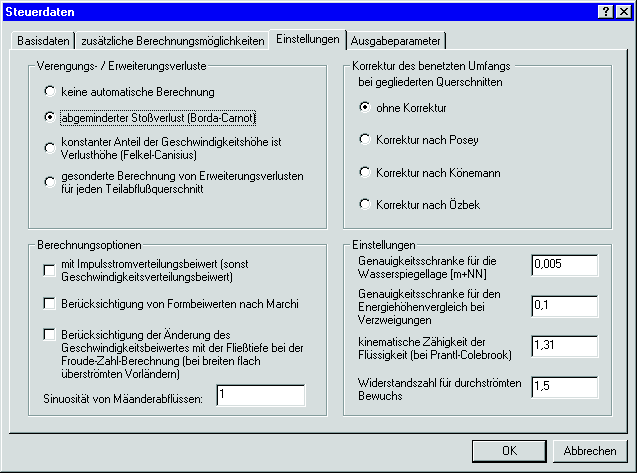
\includegraphics[width=1.0\textwidth]{Einstellungen}
   \caption{Registerkarte \dialog{Einstellungen} in der Dialogmaske \dialog{Steuerdaten}}
   \label{Fortgeschrittene Abb Einstellungen}
\end{figure}

\subsubsection{Verengungs-/Erweiterungsverluste}
Bez\"{u}glich der Ber\"{u}cksichtigung von Verengungs-/Erweiterungsverlusten stehen im Programm vier verschiedene M\"{o}glichkeiten
zur Verf\"{u}gung (vgl. auch Abschnitt~\ref{Fortgeschrittene Subsec Einzelverluste}):
\begin{description}
   \item[Keine automatische Berechnung:] Alle positiv in die Verlustdatei eingegebenen Werte werden als
      Verlustbeiwerte $\zeta$ im Sinne von Gleichung~\ref{Fortgeschrittene Gl Einzelverluste} interpretiert.
   \item[Abgeminderter Sto{\ss}verlust (\autor{Borda-Carnot}):] Die \"{o}rtlichen Verluste werden in Ab\-h\"{a}n\-gigkeit von der
      Geschwindigkeitsh\"{o}hendifferenz $dh_k$ folgenderma{\ss}en berechnet:
      \begin{description}
         \item [Erweiterung, $dh_k < 0$:]
            Die Verluste werden nach dem Ansatz von \autor{Borda-Car\-not}
            (Gleichung~\ref{Fortgeschrittene Gl VerlustBordaCarnot}) f\"{u}r eine Querschnittsaufweitung berechnet. Ein
            positiv in die Verlustdatei eingegebener Wert fungiert dabei als Abminderungsfaktor $c_i$ f\"{u}r den Sto{\ss}verlust.
         \item [Verengung, $dh_k \geq 0$:]
            Die Verluste an Stellen, an denen der Querschnitt eingeengt wird, werden nicht ber\"{u}cksichtigt, solange in der
            Verlustdatei an dieser Stelle kein Wert steht. Ein positiver Wert in der Verlustdatei am stromauf gelegenen
            Profil wird vom Programm als Verlustbeiwert $\zeta$ interpretiert und die Verlusth\"{o}he nach
            Gleichung~\ref{Fortgeschrittene Gl Einzelverluste} berechnet.
      \end{description}

      Soll der \"{o}rtliche Verlust \"{u}ber das Fl\"{a}chenverh\"{a}ltnis abgesch\"{a}tzt werden, so mu{\ss} in der Verlustdatei an dieser Stelle ein negativer Wert stehen. Der Betrag dieses Wertes wird dann als Abminderungsfaktor $c_i$ im Sinne von Gleichung~\ref{Fortgeschrittene Gl Verengungsverluste} gedeutet.

   \item [Konstanter Anteil der Geschwindigkeitsh\"{o}he ist Verlusth\"{o}he (\autor{Felkel-Canisius}):]
         Im Programm WSPLWA wird in Anlehnung an \cite{FelkelCanisius} die
         Geschwindigkeitsverteilung bei der Berechnung der Geschwindigkeitsh\"{o}he ber\"{u}cksichtigt. Der
         Geschwindigkeitsverteilungsbeiwert $\alpha$ wird n\"{a}herungsweise entsprechend Gleichung~\ref{Einstieg Gl
         Geschwindigkeitsverteilung} aus den mittleren Geschwindigkeiten im Flu{\ss}bett und den Vorl\"{a}ndern berechnet, wobei
         die Geschwindigkeitsverteilung in den Teilstromr\"{o}hren selbst durch Ansatz von $\alpha_j = 1$ vernachl\"{a}ssigt wird.
         Der kinetische Energieanteil bzw. die Geschwindigkeitsh\"{o}he wird damit n\"{a}herungsweise aus
         \begin{equation}
            h_k = \frac{\sum \left( v_j^3 \cdot A_j \right)}{2g \cdot Q}
         \end{equation}
         berechnet. Bei Wahl des Ansatzes nach \autor{Felkel-Canisius} wird bei geringeren Flie{\ss}geschwindigkeiten
         ein konstanter Anteil der Geschwindigkeitsh\"{o}hendifferenz als Verlusth\"{o}he angenommen. %Dieser betr\"{a}gt:
%         \begin{equation}
%            H_{ZV} = 2/3 \cdot h_k
%         \end{equation}
         Nimmt die Flie{\ss}geschwindigkeit im Unterwasser zu, so errechnen sich die Verluste im jeweiligen Profil mit Hilfe der
         in der Verlustdatei angegeben Werte nach Gleichung~\ref{Fortgeschrittene Gl Einzelverluste}.
   \item [Gesonderte Berechnung von Erweiterungsverlusten f\"{u}r jeden Teilabflu{\ss}querschnitt:] Bei der gesonderten Berechnung
         der Erweiterungsverluste nach~\cite{KnaufKoennemann} werden f\"{u}r jeden Teilabflu{\ss}querschnitt die Verlusth\"{o}hen mit
         Hilfe der mittleren lokalen Geschwindigkeit im Teilabflu{\ss}querschnitt ermittelt.
\end{description}

\begin{hinweis}
Da die Interpretation der Werte aus der Verlustdatei sowohl von den eingestellten Berechnungsoptionen, als 	auch von den berechneten Geschwindigkeitsh�hen ab\-h�n\-gig ist, sollte immer zun�chst ein erster Berechnungslauf ohne Angabe zu\-s�tz\-li\-cher �rtlicher Verluste mit den voreingestellten Optionen erfolgen.Auf der Grundlage der so erhaltenen Geschwindigkeitsh�hen k�nnen dann gezielt Verlustbeiwerte in die Verlustdatei eingegeben werden.
\end{hinweis}

\subsubsection{Froudezahlberechnung}
Bei praktischen Anwendungen des Rechenprogrammes hat sich gezeigt, da{\ss} die aus
\begin{equation}
   \frac{d H_E}{d h} = \frac{d(W + v_m^2/2g)}{dh}
\end{equation}
mit der N\"{a}herung $\alpha=\mathrm{konstant}$ abgeleitete Gleichung~\ref{Einstieg Gl Froudezahl} f\"{u}r die \autor{Froude}-Zahl
bei sehr breiten Vorl\"{a}ndern und kleinen Flie{\ss}tiefen unrealistisch hohe Werte liefert. Die \"{A}nderung des
Geschwindigkeitsh\"{o}henbeiwertes mit der Flie{\ss}tiefe kann nicht mehr vernachl\"{a}ssigt werden, wenn sich die Abflu{\ss}verteilung im
Flie{\ss}querschnitt mit der Flie{\ss}tiefe sehr stark \"{a}ndert. Dies ist bei breiten, nur flach \"{u}berstr\"{o}mten Vorl\"{a}ndern der Fall.
Ber\"{u}cksichtigt man den Einflu{\ss} der Flie{\ss}tiefenabh\"{a}ngigkeit von $\alpha$, so kommt man nach~\cite{KnaufKoennemann} zu
folgender Absch\"{a}tzung f\"{u}r die \autor{Froude}-Zahl:
\begin{equation}
   \label{Fortgeschrittene Gl Froudezahl}
   Fr = Q \cdot \sqrt{\frac{3 \cdot Z_E \cdot N_E' - N_E \cdot Z_E'}{N_E^4 \cdot 2g}}
\end{equation}
\begin{eqnarray*}
   \textrm{mit} \quad Z_E &=& A_L \cdot v_L^3 + A_F \cdot v_F^3 + A_R \cdot v_R^3 \\
                      Z_E'&=& c_E \cdot (b_L \cdot v_L^3 + b_F \cdot v_F^3 + b_R \cdot v_R^3) \\
                      N_E &=& v_L \cdot A_L + v_F \cdot A_F + v_R \cdot A_R \\
                      N_E'&=& c_N \cdot (v_L \cdot b_L + v_F \cdot b_F + v_R \cdot b_R)
\end{eqnarray*}
\begin{quote}
   Entsprechend dem jeweiligen Flie{\ss}gesetz sind f\"{u}r die Ableitungskonstanten $c_E$ und $c_N$ folgende Werte einzusetzen:
   \begin{quote}
      \begin{tabular}{lcc}
         \autor{Manning-Strickler}  &  $\quad c_E = 3,0$   &  $\quad c_N = 1,66$  \\
         \autor{Prandtl-Colebrook}  &  $\quad c_E = 2,5$   &  $\quad c_N = 1,50$
      \end{tabular}
   \end{quote}
\end{quote}
Eine generelle Anwendung von Gleichung~\ref{Fortgeschrittene Gl Froudezahl} zur Berechnung der \autor{Froude}-Zahl ist
m\"{o}g\-lich. Da in der Praxis bisher meist nur Gleichung~\ref{Einstieg Gl Froudezahl} verwendet wird, wird die aufwendigere
Gleichung~\ref{Fortgeschrittene Gl Froudezahl} im Rechenprogramm nur bei Eingabe eines entsprechenden Steuerparameters
\checkbox{Ber\"{u}cksichtigung der \"{A}nderung des Geschwindigkeitsbeiwertes mit der Flie{\ss}tiefe bei der Froude-Zahl-Berechnung}
verwendet. Die \autor{Froude}-Zahl geht nicht direkt in die Berechnung der Wasserspiegellagen ein, sie dient lediglich zur
Ermittlung und Kennzeichnung des Flie{\ss}zustandes.


\subsubsection{Zusatzparameter}
Unter der Registerkarte \dialog{Einstellungen}, k\"{o}nnen verschiedene f\"{u}r die Berechnung relevante Parameter, die
standardm\"{a}{\ss}ig vorbesetzt sind, editiert werden. Eine \"{A}nderung der voreingestellten Werte ist im allgemeinen nicht
erforderlich.
\begin{description}
   \item[Genauigkeitsschranke f\"{u}r die Wasserspiegellage:] ~\newline
      Die Genauigkeitsschranke f\"{u}r die Wasserspiegellagenberechnung ist im Programm auf
      \mbox{$\mathit{EPSH} = 0,005\unit{m}$} voreingestellt.
   \item[Genauigkeitsschranke f\"{u}r den Energieh\"{o}henvergleich bei Verzweigungen:] ~\newline
      Der Ab\-bruch der iterativen Berechnungen an Verzweigungen erfolgt bei Unterschreitung der Genauigkeitsschranke
      $\mathit{EPSV}$f\"{u}r den Energieh\"{o}henvergleich an der Verzweigungsstelle. Diese ist auf $0,10\unit{m}$ voreingestellt.
%      Die Ge\-nauig\-keitsschranke f\"{u}r den Abbruch der iterativen Berechnung bei Verzweigungen ist mit \mbox{$\mathit{EPSV} =
%      0,01\unit{m}$} vorbelegt.
   \item[kinematische Z\"{a}higkeit der Fl\"{u}ssigkeit:] ~\newline
      Die kinematische Z\"{a}higkeit einer Fl\"{u}ssigkeit ist von der Temperatur der Fl\"{u}ssigkeit abh\"{a}ngig. Voreingestellt ist die
      kinematischen Z\"{a}higkeit von Wasser bei einer Temperatur von 10\grad C:
      \begin{equation*}
         \nu = 1,31 \cdot 10^{-6}\unit{m^2/s}
      \end{equation*}
      Der Wert der kinematische Z\"{a}higkeit wird programmintern mit $10^{-6}$ multipliziert.
   \item[Widerstandszahl f\"{u}r durchstr\"{o}mten Bewuchs:] ~\newline
      In der Standardeinstellung betr\"{a}gt die Widerstandszahl f\"{u}r
      durchstr\"{o}mten Bewuchs $c_{WR} = 1,5$. Der Zahlenbereich f\"{u}r die Eingabe ist auf $1.0 < c_{WR} < 1.6$ eingeschr\"{a}nkt.
\end{description}

\subsubsection{Sinuosit\"{a}t}
\autor{Chow}~\cite{Chow} empfiehlt den \autor{Manning-Strickler}-Beiwert bei M\"{a}andrierung eines Gew\"{a}s\-sers zu erh\"{o}hen.
Kennzeichnende Gr\"{o}{\ss}e ist hierbei die Sinousit\"{a}t $S_M$ eines M\"{a}anders:
\begin{eqnarray*}
   \begin{minipage}{0.40\textwidth}
      \hspace{0.5cm}
      
\includegraphics{Maeander}
   \end{minipage}
   \begin{minipage}{0.6\textwidth}
      \begin{equation}
         S_M = \frac{\textrm{Talweg des M"aanders}}{\textrm{Wellenl"ange des M"aanders}}
      \end{equation}
      \\ \\
   \end{minipage}
\end{eqnarray*}
Nach~\cite{BWK1999} kann die Empfehlung von~\autor{Chow} in einen Korrekturfaktor zum Widerstandsbeiwert $\lambda$ bei
Kompaktquerschnitten wie folgt umgesetzt werden:
\begin{equation}
   \lambda_{ges,M} = c_{M,K} \cdot \lambda_{ges}
\end{equation}
\begin{quote}
   \textrm{mit} \qquad
   \begin{tabular}{lll}
      $c_{M,K} = 6,40 \cdot S_M - 5,40$   &  f\"{u}r   &  $1,00 < S_M \leq 1,05$ \\
      $c_{M,K} = 0,822 \cdot S_M + 0,45$  &  f\"{u}r   &  $1,05 < S_M \leq 1,50$ \\
      $c_{M,K} = 1,69$                    &  f\"{u}r   &  $1,50 < S_M$
   \end{tabular}
\end{quote}
Bei gegliederten Querschnitten erh\"{o}ht sich der Korrekturfaktor nach~\cite{BWK1999} entsprechend
\begin{equation}
   c_{M,G} = 1,0 + (2,5 \cdot c_{M,K} - 1,0)
\end{equation}
Die Verwendung von pauschalen Faktoren zur Erh\"{o}hung der Reibungsbeiwerte k\"{o}nnen dem tats\"{a}chlichen Einflu{\ss} einer
M\"{a}andrierung nur n\"{a}herungsweise Rechnung tragen. Bei starker M\"{a}andrierung oder besonderen Genauigkeitsanforderungen ist
der Anwendungsbereich einer eindimensionalen Str\"{o}mungsberechnung nicht mehr gegeben.

\subsubsection{Formbeiwert nach Marchi}
Das Widerstandsgesetz von \autor{Prandtl-Colebrook} wurde f\"{u}r Rohrstr\"{o}mungen mit \"{u}ber den benetzten Umfang gleichm\"{a}{\ss}ig
verteilten Wandschubspannungen entwickelt. Bei Gerinnestr\"{o}mungen mit freiem Wasserspiegel ist diese Voraussetzung nicht
gegeben.

Bei Kompaktquerschnitten entstehen Sekund\"{a}rstr\"{o}mungen, die eine ungleichm\"{a}{\ss}ige Geschwindigkeitsverteilung und eine
ungleichm\"{a}{\ss}ige Wandschubspannungsverteilung verursachen. Zum Ausgleich dieser Abweichungen ist das einparametrige
Formbeiwertkonzept von \autor{Marchi} \cite{SchroederRCM2} bei einer eindimensionalen Str\"{o}mungsberechnung zu empfehlen.
Bei diesem Konzept wird mit einer Korrektur des f\"{u}r die Wandschubspannung repr\"{a}sentierenden hydraulischen Radius
gearbeitet:
\begin{equation}
   d_{\mathit{eff}} = f \cdot d = f \cdot 4 \cdot r_{hy}
\end{equation}
Diese Korrektur ver\"{a}ndert die Konstanten der \autor{Prandtl-Colebrook}-Formel:
\begin{equation*}
   C_1 = 2,51 / f    \quad  \textrm{und}  \quad C_2 = 3,71 \cdot f
\end{equation*}

Nat\"{u}rliche Flie{\ss}querschnitte k\"{o}nnen am einfachsten durch hydraulisch gleichwertige Rechteckquerschnitte angen\"{a}hert werden.
F\"{u}r rechteckige Querschnitte ergibt sich ein Formbeiwert zwischen $f = 0,52$ (sehr breite Querschnitte $h/b \Rightarrow
0$) und $f = 0,9$ (Quadrat). Durch die Formbeiwerte ver\"{a}ndern sich die Zahlenwerte der Prandtl-Colebrook-Formel wie in
Tabelle~\ref{Fortgeschrittene Tab FormbeiwertMarchi} angegeben.

\begin{table}[hbt]
   \centering
   \input{Fortgeschrittene/tab/FormbeiwertMarchi.tab}
   \caption{Formbeiwerte nach Marchi}
   \label{Fortgeschrittene Tab FormbeiwertMarchi}
\end{table}

Als Bestimmungsgleichung f\"{u}r den Formbeiwert beliebiger Rechtecke ist in \cite{SchroederRCM2} folgende Sch\"{a}tzformel
angegeben:
\begin{equation}
   f = 0,09 - 0,38 \cdot e^{-5h/b}
\end{equation}
F\"{u}r teilgef\"{u}llte Kreisquerschnitte hat \autor{Bock} Formbeiwerte zwischen 0,4 und 1,0 gemessen. Eine polynomische
Anpassung der Me{\ss}werte f\"{u}hrt auf folgende Bestimmungsgleichung f\"{u}r Formbeiwerte beim teilgef\"{u}llten Kreisquerschnitt:
\begin{equation}
   f = 0,3458 + 2,2026 \cdot \frac{h}{d} - 2,4566 \cdot \left( \frac{h}{d} \right)^2
       + 0,9084 \cdot \left( \frac{h}{d} \right)^3
\end{equation}

\subsubsection{Korrektur des benetzten Umfangs}
Eine ungleichm\"{a}{\ss}ige Geschwindigkeitsverteilung in einem Flie{\ss}querschnitt vermindert die hydraulische Leistungsf\"{a}higkeit,
da das Reibungsgef\"{a}lle linear mit dem Geschwindigkeitsverteilungsbeiwert zunimmt. Bei gegliederten Querschnitten
vergr\"{o}{\ss}ert sich das Energieliniengef\"{a}lle weiterhin durch zus\"{a}tzliche Interaktionswiderst\"{a}nde an den Trennfl\"{a}chen zwischen
den Vorl\"{a}ndern mit kleiner Flie{\ss}geschwindigkeit und dem Flu{\ss}schlauch mit gr\"{o}{\ss}erer Flie{\ss}geschwindigkeit.

Zum Ausgleich dieser zus\"{a}tzlichen Flie{\ss}widerst\"{a}nde wird in der Fachliteratur eine Vergr\"{o}{\ss}erung des benetzten Umfanges im
Flu{\ss}schlauch unter Beibehaltung der hydraulischen Radien im Vorland empfohlen. Nach Untersuchungen von
\autor{Kradolfer}~\cite{Kradolfer} und \autor{Knauf}~\cite{Knauf1} kann diese Korrektur zu unsinnigen Ergebnissen f\"{u}hren,
wenn sie ohne Beachtung der zul\"{a}ssigen Anwendungsgrenzen angewendet wird. Im Programmsystem stehen drei verschiedene
Korrekturm\"{o}glichkeiten zur Verf\"{u}gung:
\begin{description}
   \item[Korrektur nach Posey:] Nach Untersuchungen von \autor{Posey} im Jahre 1967 \cite{Kradolfer} nimmt der
      Korrekturbedarf mit zunehmender Flie{\ss}tiefe im Vorland ab. Bei Verh\"{a}ltnissen \mbox{$h_V > 0,5 h_F$} sollten auch
      gegliederte Flie{\ss}querschnitte ohne Bewuchs wie Kompaktquerschnitte berechnet werden \cite{Knauf1, ATV111}.
      Der abnehmende Einflu{\ss} des Zusatzwiderstandes kann entsprechend~\cite{ATV111} durch folgende Korrekturgr\"{o}{\ss}e zum
      benetzten Umfang des Flu{\ss}schlauchs n\"{a}herungsweise automatisch ber\"{u}cksichtigt werden:
      \begin{equation}
         \begin{split}
            U_{F,cal} &= U_F + U_{T,L} + U_{T,R} \\
            U_{F,cal} &= U_F + h_{V,L} \cdot \left( 1 - \frac{2h_{V,L}}{h_F} \right)
                         + h_{V,R} \cdot \left( 1 - \frac{2h_{V,R}}{h_F} \right)
         \end{split}
      \end{equation}
   \item[Korrektur nach K\"{o}nemann:]
      Meist wird die von \autor{K\"{o}nemann} vorgeschlagene Korrektur empfohlen~\cite{SchroederW, DVWK1991}, ohne auf die
      Anwendungsgrenzen besonders hinzuweisen. Die Korrektur besteht in der Vergr\"{o}{\ss}erung des benetzten
      Flu{\ss}schlauch-Umfanges durch die vollen Trennfl\"{a}chenh\"{o}hen, wobei die Trennfl\"{a}chenrauheit selbst in erster N\"{a}herung
      gleich der angrenzenden Wandfl\"{a}chenrauheit des Flu{\ss}schlauchs gesetzt wird.
      \begin{equation}
         U_{F,cal} = U_F + U_{T,L} + U_{T,R}  \qquad   \textrm{mit}   \qquad   k_T = k_W
      \end{equation}
      Diese Korrektur ist nur f\"{u}r kleine Vorlandflie{\ss}tiefen \mbox{$h_V < h_F/3$} zu empfehlen und nur bei gegliederten
      Gerinnen \emph{ohne} Bewuchs anwendbar.
   \item[Korrektur nach \"{O}zbek:]
      Bei kleinen Flie{\ss}tiefen im Vorland \mbox{($h_V < h_F/3$)} wird in~\cite{DVWK1991} ein Sicherheitsfaktor von mind. 3
      zur Vergr\"{o}{\ss}erung der Trennfl\"{a}chenrauheit empfohlen. Zur Verbesserung dieser unbefriedigenden Situation haben
      \autor{Bretschneider} und \autor{\"{O}zbek} (1997) anhand von Modellversuchen (SERC, Wallingford, UK) eine Sch\"{a}tzformel
      zur Ermittlung der Trennfl\"{a}chenrauheit $\lambda_T$ bei kleinen Vorland\-\"{u}berstr\"{o}mungen abgeleitet :
      \begin{equation}
         \lambda_T = 0,71 \cdot \left(\frac{b_V}{b_F} \right)^{0,48}
                     \cdot \left(\frac{h_F}{h_V} \right)^{1,05} \cdot \lambda_W
      \end{equation}
      Entsprechend den Modellversuchen werden die G\"{u}ltigkeitsgrenzen wie folgt angegeben:
      \begin{quote}
         Tiefenverh\"{a}ltnis:    \quad    $h_F/h_V > 2$, \\
         Breitenverh\"{a}ltnis:   \quad    $b_V/b_F \leq 4,56$
      \end{quote}
      Diese Korrektur ist nur bei gegliederten Gerinnen und einer Berechnung mit dem Flie{\ss}gesetz von
      \autor{Prandtl-Colebrook} \emph{ohne} Bewuchs anwendbar.
\end{description}


\subsubsection{Impulsstromverteilungsbeiwert}
In~\cite{BWK1999} wird empfohlen bei konstanten Abfl\"{u}ssen die ma{\ss}gebende Energieh\"{o}he mit Hilfe des
Geschwindigkeitsverteilungsbeiwertes zu ermitteln und bei diskontinuierlichen Abfl\"{u}ssen den Impulsstromverteilungsbeiwert
zu verwenden. Die Berechnung der ma{\ss}gebenden Energieh\"{o}he kann von \wspwin{} wahlweise mit dem
Geschwindigkeitsverteilungsbeiwert $\alpha$ nach Gleichung~\ref{Einstieg Gl Geschwindigkeitsverteilung}
(Standardeinstellung) oder, falls das entsprechende Kontrollk\"{a}stchen bet\"{a}tigt wurde, mit dem Impulsstromverteilungsbeiwert
$\alpha'$ nach Gleichung~\ref{Einstieg Gl Impulsstromverteilung} berechnet werden.

\clearpage
\subsection{Ausgabeparameter}

\begin{figure}[hbt]
   \centering
   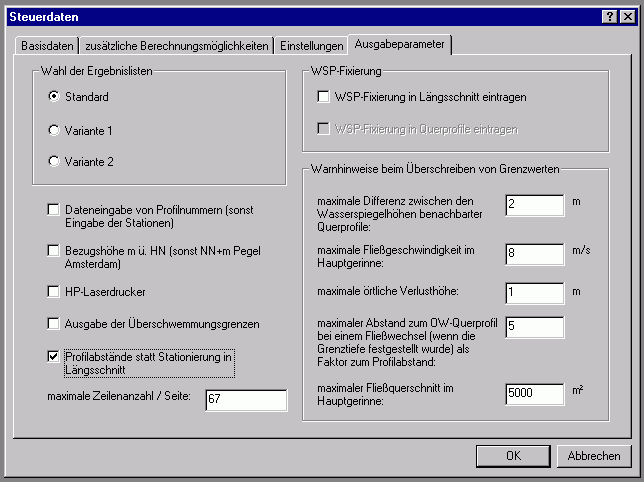
\includegraphics[width=1.0\textwidth]{Ausgabeparameter}
   \caption{Registerkarte \dialog{Ausgabeparameter} in der Dialogmaske \dialog{Steuerdaten}}
   \label{Fortgeschrittene Abb Ausgabeparameter}
\end{figure}


\subsubsection{Wahl der Ergebnislisten}
Bez\"{u}glich des Darstellungformates der Ergebnisdateien kann zwischen drei unterschiedlichen Ausgabevarianten gew\"{a}hlt
werden. Die Ausgabe der einzelnen hydraulischen Parameter, Wasserspiegellagen etc. erfolgt in Form einer Tabelle. Wenn Sie
die Voreinstellung nicht \"{a}ndern, wird das Standardformat (Abbildung~\ref{Fortgeschrittene Abb Standardausgabe}) f\"{u}r die
Ausgabe verwendet.

Die Ausgabe der Variante~1 (vgl. Abbildung~\ref{Fortgeschrittene Abb AusgabeVariante1}) enth\"{a}lt zus\"{a}tzlich zu den
Parametern der Standardausgabe die berechneten Schleppspannungen auf den Vorl\"{a}ndern und im Flu{\ss}schlauch sowie die
Verlustbeiwerte $\zeta$. Daf\"{u}r sind Geschwindigkeits-, Impulsstromverteilungsbeiwerte und Flie{\ss}fl\"{a}chen nicht in der
Ergebnisdarstellung enthalten.

Variante~2 (vgl. Abbildung~\ref{Fortgeschrittene Abb AusgabeVariante2}) stellt die Ergebnisse der Berechnung in zwei
Tabellen untereinander dar. Die erste Tabelle gibt dabei nur die Wasserspiegellage und die Energieh\"{o}he an der Station
wieder. In der zweiten Tabelle sind die hydraulischen Parameter zusammengefa{\ss}t.

%Sollten Sie \"{u}ber einen HP-Laserdrucker verf\"{u}gen, kann es vorteilhaft sein, die Zusatzoption \checkbox{HP-Laserdrucker}
%aktivieren.

\begin{sidewaysfigure}[hbt]
   \centering
   \input{Fortgeschrittene/tab/Standardausgabe.tab}
   \caption{Ergebnisdarstellung bei der Standardausgabe}
   \label{Fortgeschrittene Abb Standardausgabe}
\end{sidewaysfigure}
\begin{sidewaysfigure}[hbt]
   \centering
   \input{Fortgeschrittene/tab/AusgabeVariante1.tab}
   \caption{Ergebnisdarstellung der Variante~1}
   \label{Fortgeschrittene Abb AusgabeVariante1}
\end{sidewaysfigure}
\begin{sidewaysfigure}[hbt]
   \centering
   \input{Fortgeschrittene/tab/AusgabeVariante2.tab}
   \caption{Ergebnisdarstellung der Variante~2}
   \label{Fortgeschrittene Abb AusgabeVariante2}
\end{sidewaysfigure}

\clearpage
\subsubsection{Profilnummern}
Anstelle der Stationierung konnten in der ehemaligen DOS-Version die Profilnummern ausgedruckt werden. Es war dann die
entsprechende Option einzugeben, die in der Windows-Version keine Bedeutung mehr besitzt.

\subsubsection{Bezugsh\"{o}he}
Als Bezugsh\"{o}he f\"{u}r den tabellarischen Ergebnisausdruck kann wahlweise der Pegel Amsterdam  oder der Pegel Kronstadt
gew\"{a}hlt werden. In letzterem Fall ist das K\"{a}stchen \checkbox{Bezugsh\"{o}he m \"{u}. HN} auf der Registerkarte
\dialog{Ausgabeparameter} zu markieren.
\begin{quote}
   \begin{tabular}{lll}
      \textbf{Pegel}    &  \textbf{H\"{o}henangabe} \\[3pt]
      Amsterdam: \qquad  &  NN+m \\
      Kronstadt:        &  m \"{u} HN
   \end{tabular}
\end{quote}
Die Berechnung ist nicht an die Wahl eines der beiden H\"{o}henbezugssysteme gebunden. Sie k\"{o}nnen bei der Eingabe der Daten
jede beliebige Referenzh\"{o}he verwenden. Die Einheiten sind dann ggf. im Ergebnisausdruck von Hand anzupassen.


\subsubsection{Ausgabe von \"{U}berschwemmungsgrenzen}
%Scheint nicht zu funktionieren.
Durch Aktivieren der Option \checkbox{Ausgabe der \"{U}berschwemmungsgrenzen} werden diese in einer eigenen Datei im
Projektunterverzeichnis \datei{...\textbackslash dath} ihres aktuelles Projektes gepeichert. Der vierte und f\"{u}nfte
Buchstabe des Dateinamens lautet \datei{*ug*.*}, beispielsweise enth\"{a}lt die Datei \datei{fuug0001.001} die
\"{U}berschwemmungsgrenzen einer Berechnung an der Fulda.

\subsubsection{HP-Laserdrucker}
Verwenden Sie einen HP-Laserdrucker zur Ausgabe der Berechnungsergebnisse, so kann es von Vorteil sein, wenn diese Option
markiert wird.

\subsubsection{Zeilenanzahl}
\"{U}ber ein Editierfeld kann die vorgegebene Zeilenanzahl im Resultatausdruck ge\"{a}ndert werden. Standardm\"{a}{\ss}ig werden in der
Ergebnisdatei 67~Zeilen/Seite dargestellt. Sollten Sie mehr oder weniger Zeilen darstellen m\"{o}chten, k\"{o}nnen Sie die
entsprechende \"{A}nderung hier vornehmen.


\subsubsection{Wasserspiegelfixierungen}
Unter dem Men\"{u}punkt Zustand (vgl. Abschnitt~\ref{Einstieg Subsec Abflussdatei}) haben Sie die M\"{o}glichkeit, f\"{u}r einzelne
Abflu{\ss}ereignisse gemessene Wasserspiegellagen an den jeweiligen Stationen einzutragen. Wenn Sie m\"{o}chten, da{\ss} diese
Wasserspiegelfixierungen im Rahmen der Berechnung automatisch in die Querprofile und L\"{a}ngsschnitte mit eingetragen werden,
so markieren Sie \checkbox{WSP-Fixierung in L\"{a}ngsschnitt eintragen}. Der Eintrag in die Querprofile kann erst vorgenommen
werden, wenn der Eintrag in den L\"{a}ngsschnitt aktiviert ist.

\clearpage
\subsubsection{Warnhinweise beim \"{U}berschreiten von Grenzwerten}
\wspwin{} gibt bei der \"{U}berschreitung von Grenzwerten Warnungen im Ergebnisausdruck aus. Im Fall der Standardeinstellungen
erfolgt eine Warnung, wenn
\begin{itemize}
   \item die Differenz der Wasserspiegelh\"{o}hen in benachbarten Querprofilen $2,0\unit{m}$ \"{u}berschreitet,
   \item die maximale Flie{\ss}geschwindigkeit im Hauptgerinne gr\"{o}{\ss}er als $8,0\unit{m/s}$ ist,
   \item die \"{o}rtliche Verlusth\"{o}he den Wert von $1,0\unit{m}$ erreicht,
   \item der Abstand des oberwasserseitigen Querprofils bei einem Flie{\ss}wechsel gr\"{o}{\ss}er als der f\"{u}nffache Profilabstand wird,
   \item der Flie{\ss}querschnitt die Grenze von $5000\unit{m^2}$ \"{u}berschreitet.
\end{itemize}


\subsection{Massenberechnung}

\wspwin{} kann mit einem Zusatzmodul zur Massenberechnung geliefert werden. Berechnet werden im einzelnen:
\begin{itemize}
   \item Auf- und Abtragsfl\"{a}che sowie die daraus resultierende Fl\"{a}chendifferenz f\"{u}r alle Stationen, differenziert nach
       linkem/rechtem Vorland und Hauptgerinne. Die Differenzierung in Vorl\"{a}nder und Flu{\ss}schlauch erfolgt anhand der
       Trennfl\"{a}chen bzw. B\"{o}schungsoberkanten des Referenzzustandes.
   \item Massenberechnung f\"{u}r einzelne Berechnungsabschnitte unterteilt f\"{u}r Vorl\"{a}nder und Flu{\ss}schlauch. Positive Werte
      kennzeichnen Auf-, negative Abtrag. Das Volumen ergibt sich aus Multiplikation der Fl\"{a}chendifferenz mit der L\"{a}nge des
      Berechnungsabschnitts.
      \begin{equation}
         \begin{minipage}{0.45\linewidth}
            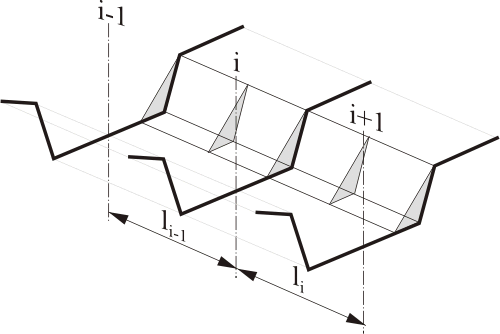
\includegraphics[width=1.0\linewidth]{Massenberechnung}
         \end{minipage}
         \qquad \Delta V_i = \Delta A_i \cdot \frac{l_{i-1} + l_i}{2}
      \end{equation}
   \item Masse der Einzelabschnitte
   \item resultierende Gesamtmasse
\end{itemize}
Voraussetzungen f\"{u}r die Durchf\"{u}hrung einer Massenberechnung zwischen zwei Zust\"{a}n\-den sind der gleiche Gew\"{a}ssername im
Referenz- und Vergleichszustand und Profile mit gleichen Stationsangaben sowie identischen Gel\"{a}ndekoordinaten am jeweils
ersten und letzten Profilpunkt. Parallel zur Massenberechnung kann auch  eine Gel\"{a}ndeverkn\"{u}pfung bzw. Fl\"{a}chenberechnung
nach Abschnitt~\ref{Fortgeschrittene Subsec Vergleichszustaende} durchgef\"{u}hrt werden. Dies erm\"{o}glicht es, die Gel\"{a}ndeh\"{o}hen
der einzelnen Profile im Referenz- und Vergleichszustand direkt (auch optisch) zu vergleichen.
\begin{sidewaysfigure}[hbt]
   \centering
   \input{Fortgeschrittene/tab/Massenberechnung.tab}
   \caption{Ergebnis der Massenberechnung}
   \label{Fortgeschrittene Abb Massenberechnung}
\end{sidewaysfigure}

Um den Massenunterschied zwischen zwei unterschiedlichen Ausbauzust\"{a}nden eines Gew\"{a}ssers zu ermitteln, w\"{a}hlen Sie die
Men\"{u}folge \menu{\marrow \underline{B}erechnung \marrow \underline{M}assenberechnung}. Sie m\"{u}ssen nun zun\"{a}chst den
Referenzzustand und den Vergleichszustand ausw\"{a}hlen. Danach wird die Massenberechnung gestartet. Die Ergebnisse werden in
im Unterverzeichnis \datei{...\textbackslash dath} Ihres Projektverzeichnisses unter dem Dateinamen \datei{masse.txt}
abgelegt. Dabei wird eine bereits bestehende Ergebnisdatei \"{u}berschrieben. Die Datei kann im Editor eingesehen werden. Der
Aufruf erfolgt \"{u}ber das Men\"{u} \menu{\marrow \underline{E}rgebnisse \marrow Ergebnisse der \underline{M}assenberech\-nung}.
\begin{hinweis}
   M\"{o}chten sie die Ergebnisse einer fr\"{u}heren Massenberechnung im gleichen Projekt nicht \"{u}berschreiben, so speichern sie
   die Datei \datei{masse.txt} vor einer erneuten Berechnung unter einem anderen Namen.
\end{hinweis}


\subsection{Sonderprogramme station\"{a}r gleichf\"{o}rmig}

Aus \wspwin{} heraus k\"{o}nnen Sonderprogramme des Programmsystems HYDRA u.a. zu station\"{a}r gleichf\"{o}rmigen Berechnungen
aufgerufen werden. Es handelt sich hierbei um DOS-Programme, die in einem DOS-Fenster ablaufen. Folgende Programme sind
(sofern erworben) verf\"{u}gbar:
\begin{itemize}
   \item Wehre
   \item Rohre
   \item Gerinne
   \item Stra{\ss}enbau
   \item Entlastungsbauwerke
\end{itemize}
Weitere Angaben hierzu finden Sie im Kapitel~\ref{Dialogprogramme}.




\clearpage
%%%%%%%%%%%%%%%%%%%%%%%%%%%%%%%%%%%%%%%%%%%%%%%%%%%%%%%%%%%%%%%%%%%%%%%%%%%%%%%%%%%%%%%%%%%%%%%%%%%%%%%%%%%%%%%%%%%%%%%%%%%%
\section{Ergebnisse einsehen}
%%%%%%%%%%%%%%%%%%%%%%%%%%%%%%%%%%%%%%%%%%%%%%%%%%%%%%%%%%%%%%%%%%%%%%%%%%%%%%%%%%%%%%%%%%%%%%%%%%%%%%%%%%%%%%%%%%%%%%%%%%%%

Im Rahmen der Bearbeitung mit \wspwin{} werden die nachfolgend aufgef\"{u}hrten Ergebnisdateien im Projektunterverzeichnis
\datei{...\textbackslash dath} erstellt. Der Dateiname leitet sich im allgemeinen aus dem Namen der zugrunde gelegten
Berechnungsvariante ab, wobei lediglich die dritten und vierten Buchstaben modifiziert werden. F\"{u}r eine
Berechnungsvariante an der Fulda \datei{fu000001.001} erg\"{a}ben sich folgende Ergebnisdateien: \\ ~ \\

\input{Fortgeschrittene/tab/Ergebnisdateien.tab}


\subsection{L\"{a}ngsschnitte einsehen und vergleichen}

Nach der Berechnung k\"{o}nnen die Ergebnisse in einer L\"{a}ngsschnittgrafik eingesehen werden (Abschnitt~\ref{Einstieg Subsec
Laengsschnitteditor}). Die Darstellung l\"{a}{\ss}t sich bearbeiten. So macht es beispielsweise Sinn, bei verzweigten Systemen
einzelne Profilpunkte zu l\"{o}schen, um eine eindeutige Darstellung zu erhalten. Sie entfernen nicht mehr ben\"{o}tigte Stationen
aus der Grafik, indem sie die zugeh\"{o}rigen $y$-Werte l\"{o}schen. Sowohl die Profildatei als auch die Grafik werden dann
aktualisiert.

Die Datens\"{a}tze \afz{Text} und \afz{Bauwerk} k\"{o}nnen nicht \"{u}ber \wspwin{} editiert werden. Das L\"{o}schen der kompletten
Datens\"{a}tze ist allerdings m\"{o}glich. Diese Datenblocktypen sind lediglich f\"{u}r das sp\"{a}tere Plotten relevant.

Beim Einsehen des L\"{a}ngsschnitts besteht ferner die M\"{o}glichkeit, verschiedene Berechnungsvarianten zu vergleichen. W\"{a}hlen
Sie hierzu aus dem L\"{a}ngsschnitteditor heraus die Men\"{u}folge \menu{ \marrow Ergebnisse \marrow L\"{a}ngsschnitt vergleichen}.
Sie werden dazu aufgefordert, eine weitere Berechnungsvariante auszuw\"{a}hlen. Sobald Sie eine Variante ausgew\"{a}hlt haben,
werden aus dieser Datei die Datens\"{a}tze \afz{Sohlh\"{o}he}, \afz{B\"{o}schung li.} , \afz{B\"{o}schung re.} und der \afz{Wasserspiegel}
als \afz{2.~Sohlh\"{o}he}, \afz{2.~Wasserspiegel} etc. in ihre aktuelle L\"{a}ngsschnittdatei eingef\"{u}gt.

Bei jedem Aufruf des L\"{a}ngsschnitteditors erscheint die Meldung \afz{Es existiert bereits eine L\"{a}ngsschnittdatei.
\"{U}berschreiben?}. Ein \"{U}berschreiben der L\"{a}ngsschnittdatei ist dann sinnvoll, wenn Sie die Datei komplett neu aus den
Berechnungsergebnissen erstellen lassen wollen. Haben Sie hingegen bereits in der Datei gespeicherte Stempeldaten und
Plotinformationen eingegeben, so kann die alte L\"{a}ngsschnittdatei erhalten bleiben.


\clearpage
\subsection{Berechnungsergebnisse auswerten}
\wspwin{} verf\"{u}gt \"{u}ber drei Auswerteprogramme, mit denen es m\"{o}glich ist, sich Listen von Auswertungen der
Berechnungsergebnisse erstellen zu lassen.

\subsubsection{Listenauswertung}
Das Modul WSPLIST wertet \"{U}berflutung und Vollf\"{u}llung der Gew\"{a}sser aus. Hierzu mu{\ss} die automatische Berechnung einer
Abflu{\ss}kurve mit fester Schrittweite vorliegen. Die Definition des bordvollen Abflusses orientiert sich dabei an folgenden
Gr\"{o}{\ss}en:
\begin{itemize}
   \item erster und letzter Profilpunkt
   \item Grenzen der durchstr\"{o}mten Bereiche
   \item bei geschlossenen Durchl\"{a}ssen der h\"{o}chste Punkt
   \item bei \"{u}berstr\"{o}mten Durchl\"{a}ssen die \"{U}berstr\"{o}mungsh\"{o}he
   \item bei offenen Profilen die Lage der Trennfl\"{a}chen (hierdurch k\"{o}nnen wahlweise bordvolle Abfl\"{u}sse des Flu{\ss}schlauchs
      oder des Gesamtquerschnitts mit Vorl\"{a}ndern definiert werden)
\end{itemize}
Im Men\"{u} \menu{\marrow \underline{E}rgebnisse} finden Sie das Untermen\"{u} \menu{\marrow Auswer\underline{t}en \marrow
Beispie\underline{l}listen}. Nach dessen Aufruf erscheint zun\"{a}chst der Dialog zur Auswahl von Berechnungsvarianten. Mit
\schalter{Berechnung} wird das Auswerteprogramm gestartet. Nach der Auswertung werden Ihnen automatisch die Ergebnisse im
\wspwin{}-Editor angezeigt. Sie k\"{o}nnen die Ergebnisse auch sp\"{a}ter jederzeit \"{u}ber den Editor einsehen. \newline Folgende
Ergebnisdateien werden erstellt:
\begin{description}
   \item[\datei{*wk*.*}:] Enth\"{a}lt eine Liste aller Profile geordnet nach Abfl\"{u}ssen, mit Wassertiefe und
            Wasserspiegelbreite (Abbildung~\ref{Fortgeschrittene Abb DateiWK}).
   \item[\datei{*ue*.*}:]  Enth\"{a}lt eine Liste aller Abfl\"{u}sse geordnet nach Stationen mit \"{U}berlastungen links und rechts
            (Abbildung~\ref{Fortgeschrittene Abb DateiUE}).
   \item[\datei{*ma*.*}:] Wertet die Ergebnisdateien soweit aus, da{\ss} nur der bordvolle Abflu{\ss} $Q_{voll}$ im Profil in der
      Liste steht (Abbildung~\ref{Fortgeschrittene Abb DateiMA}).
   \item[\datei{*ex*.*}:] Ausgabe von L\"{a}ngsschnittdaten f\"{u}r einen Import in Excel. Die erste Zeile enth\"{a}lt die
      Abflu{\ss}ereignisse, in der ersten Spalte sind die Stationen verzeichnet.
\end{description}
\begin{figure}[hbtp]
   \centering
   \input{Fortgeschrittene/tab/DateiWK.tab}
      \caption{Datei \datei{*wk*.*} des Beispiels \afz{Testbach}}
      \label{Fortgeschrittene Abb DateiWK}
   \input{Fortgeschrittene/tab/DateiUE.tab}
      \caption{Datei \datei{*ue*.*} des Beispiels \afz{Testbach}}
      \label{Fortgeschrittene Abb DateiUE}
   \input{Fortgeschrittene/tab/DateiMA.tab}
      \caption{Datei \datei{*ma*.*} des Beispiels \afz{Testbach}}
      \label{Fortgeschrittene Abb DateiMA}
\end{figure}
Die Ergebnisse werden im Unterverzeichnis \datei{\textbackslash dath} abgelegt. Der Dateiname orientiert sich am Namen der
ersten ausgew\"{a}hlten Berechnungsvariante, deren 3. und 4. Buchstabe variiert.


\subsubsection{Vergleichslisten}
Neben dem Listenprogramm zur Auswertung von \"{U}berflutungen kann ein weiteres Zusatzmodul genutzt werden, das verschiedene
hydraulische Parameter aus bis zu drei Berechnungsvarianten miteinander vergleicht. Der Vergleich wird \"{u}ber das Men\"{u}
\menu{\marrow \underline{E}rgebnis\-se \marrow Auswer\underline{t}en \marrow \underline{V}ergleichen} initialisiert. Die
Auswahl der Berechnungsvarianten erfolgt in gleicher Weise wie beim Listenprogramm. Zus\"{a}tzlich erscheint jedoch ein
weiterer Dialog in dem sie einen oder mehrere zu vergleichenden Parameter ausw\"{a}hlen m\"{u}ssen
(Abbildung~\ref{Fortgeschrittene Abb AuswahlVergeleichswerte}). Die Ausgabe (vgl. Abbildung~\ref{Fortgeschrittene Abb
Vergleichsliste}) enth\"{a}lt neben den einzelnen Parametern an der Station auch die jeweilige Differenz zum Referenzzustand.
\begin{figure}[hbt]
   \centering
   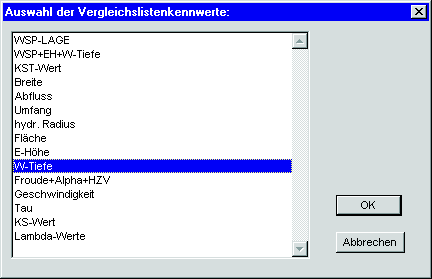
\includegraphics[width=0.8\textwidth]{AuswahlVergleichswerte}
      \caption{Dialogmaske zur Auswahl der zu vergleichenden Parameter}
      \label{Fortgeschrittene Abb AuswahlVergeleichswerte}
\end{figure}

\begin{figure}
   \centering
   \input{Fortgeschrittene/tab/Vergleichsliste.tab}
      \caption{Auszug aus einer Vergleichsliste}
      \label{Fortgeschrittene Abb Vergleichsliste}
\end{figure}

\subsubsection{Pr\"{u}flisten}
Neben der Listenauswertung und der Erstellung von Vergleichslisten existiert drittes Programm, mit dessen Hilfe aus einer
Berechnungsvariante eine Liste mit ausgew\"{a}hlten Parametern dargestellt werden kann. Nach dem Aufruf des Men\"{u}s
\menu{\marrow \underline{E}rgebnisse  \marrow Auswer\-\underline{t}en  \marrow \underline{P}r\"{u}fen  \marrow
Pr\"{u}f\underline{p}rogramm} und der Auswahl einer Berechnungsvariante wird das Pr\"{u}fprogramm gestartet. Es erscheint zun\"{a}chst
ein Dialogfenster (Abbildung~\ref{Fortgeschrittene Abb Prueflistenkennwerte}), das Sie zur Auswahl der darzustellenden
Gr\"{o}{\ss}en auffordert. Im Untermen\"{u} \menu{\marrow Voreinstellung} k\"{o}nnen Sie diese Parameter auch als Standardeinstellung
definieren. Sie werden dann bei jedem Aufruf des Pr\"{u}fprogramms als Vorauswahl angeboten.
\begin{figure}[ht]
   \centering
   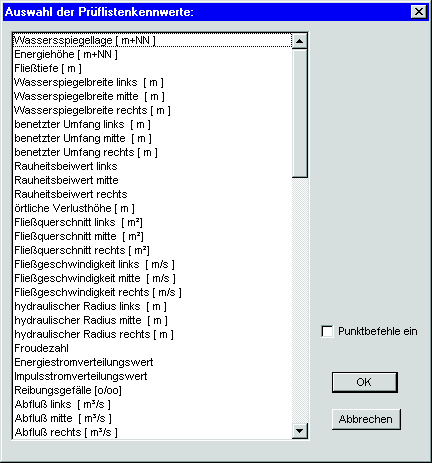
\includegraphics[width=0.8\textwidth]{Prueflistenkennwerte}
   \caption{Auswahl der Pr\"{u}flistenkennwerte}
   \label{Fortgeschrittene Abb Prueflistenkennwerte}
\end{figure}


\subsection{Wasserspiegel einf\"{u}gen}

Bei jeder Berechnung erfolgt, sofern in den Steueroptionen der Berechnung angegeben, ein Eintrag der errechneten
Wasserspiegellagen in die Querprofile. Dabei werden die bereits vorhandenen Wasserspiegellagen fr\"{u}herer Berechnungen
gel\"{o}scht.

Die Eintr\"{a}ge k\"{o}nnen auch einzeln \"{u}ber das Men\"{u} \menu{\marrow \underline{E}rgebnisse \marrow \underline{W}asserspiegel...
\marrow \underline{L}\"{o}\-schen in allen Querprofilen} aus den Querprofilen entfernt werden. In gleicher Weise lassen sich
\"{u}ber das Men\"{u} \menu{\marrow \underline{E}inf\"{u}gen in Querprofil} die Wasserspiegellagen von Berechnungsvarianten auch von
Hand in die Querprofile eingetragen. Dies ist sinnvoll, wenn kein automatischer Eintrag bei der Berechnung vereinbart
wurde, oder die Wasserspiegellagen verschiedener Varianten im Profil verglichen werden sollen.


\clearpage
%%%%%%%%%%%%%%%%%%%%%%%%%%%%%%%%%%%%%%%%%%%%%%%%%%%%%%%%%%%%%%%%%%%%%%%%%%%%%%%%%%%%%%%%%%%%%%%%%%%%%%%%%%%%%%%%%%%%%%%%%%%%
\section{Plotten}
%%%%%%%%%%%%%%%%%%%%%%%%%%%%%%%%%%%%%%%%%%%%%%%%%%%%%%%%%%%%%%%%%%%%%%%%%%%%%%%%%%%%%%%%%%%%%%%%%%%%%%%%%%%%%%%%%%%%%%%%%%%%
\begin{figure}[hbt]
   \centering
   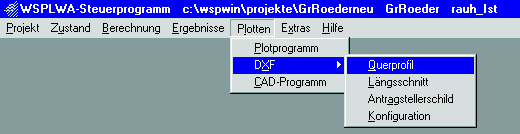
\includegraphics[width=0.8\textwidth]{MenuePlotten}
   \caption{Der Men\"{u}punkt \menu{\marrow P\underline{l}otten}}
   \label{Fortgeschrittene Abb MenuePlotten}
\end{figure}


\subsection{Plotprogramm}

Zu \wspwin{} gibt es seit 1999 ein eigenst\"{a}ndiges Plotprogramm \afz{\wspwin{}-Plotter}, \"{u}ber das Sie in einer
Windowsoberfl\"{a}che L\"{a}ngs- und Querprofile direkt formatieren und plotten k\"{o}nnen. Der Umweg \"{u}ber die Erzeugung von
\datei{*.dxf}-Dateien und ein zus\"{a}tzliches CAD-Programm entf\"{a}llt hierdurch.
Eine ausf�hrliche Beschreibung finden Sie im Handbuch des Plotprogramms.


\subsection{DXF-Dateien erzeugen}

Mit Hilfe von \wspwin{} k\"{o}nnen sowohl f\"{u}r die L\"{a}ngsschnitte, als auch f\"{u}r die Querprofile \datei{*.dxf}-Dateien erstellt
werden, die sich in einem CAD-Programm bearbeiten und plotten lassen. Vor dem Erstellen der Dateien lassen sich
verschiedene Voreinstellungen zur Art und Weise der Darstellung in der CAD-Datei vornehmen. F\"{u}r L\"{a}ngsschnitte existieren
im allgemeinen bereits Voreinstellungen aus den L\"{a}ngsschnittdateien. Bei Querprofilen sind diese komplett neu zu
erstellen.

\"{U}ber die Men\"{u}punkte \menu{\marrow P\underline{l}otten \marrow D\underline{X}F \marrow \underline{Q}uerprofil} bzw.
\menu{\marrow \underline{L}\"{a}ngsschnitt} gelangen Sie in einen Dialog zur Auswahl des Querprofils oder der
L\"{a}ngsschnittdatei. \"{U}ber die Schalter \schalter{Plotten} bzw. \schalter{OK} wird ein Programm gestartet, das die
\datei{*.dxf}-Datei aus dem markierten Profil erzeugt. Zum besseren Verst\"{a}ndnis der Eingabeparameter werden zun\"{a}chst
einige Begriffe erl\"{a}utert:
\begin{description}
   \item[Profillinie:] Sie ergibt sich aus den $(y,z)$-Koordinaten eines Datensatzes der Profildatei.
   \item[Stationslinie:] Senkrechte Linie von der Profillinie zum Schriftfeld
   \item[Schriftfeld:] Im Schriftfeld werden die Daten und Ergebnisse eingetragen. Sie dienen zur Erl\"{a}uterung der
      grafischen Darstellung
   \item[Symbole:] Alle Zeichnungseintr\"{a}ge, die durch einen Datensatz erfolgen und keine Profillinie sind, werden als
      Symbole bezeichnet.
\end{description}
Der zu erstellende Plot besteht aus drei Elementen, dem Stempel, dem Schriftfeld und der eigentlichen Zeichnung.
\begin{figure}[hbt]
   \centering
   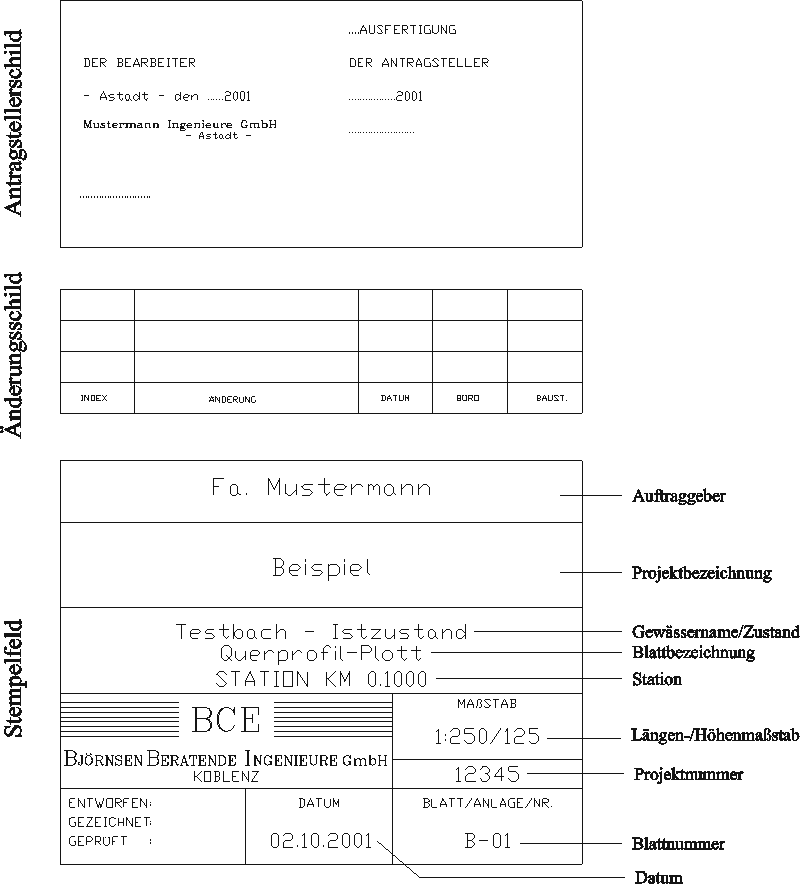
\includegraphics[width=0.9\textwidth]{Stempelfeld}
   \caption{Stempelfeld mit optionalem \"{A}nderungs- und Antragstellerschild. Zus\"{a}tzlich kann noch eine Legende dargestellt
            werden.}
   \label{Fortgeschrittene Abb Stempelfeld}
\end{figure}

\subsubsection{Stempelfeld}
In die Zeichnung wird grunds\"{a}tzlich ein Stempel (Abbildung~\ref{Fortgeschrittene Abb Stempelfeld} unten)
eingetragen. Zus\"{a}tzlich kann wahlweise ein \"{A}nderungsschild, ein Antragstellerschild oder eine Legende in die Zeichnung
aufgenommen werden. Die Definitionen der Eintragungen im Antragstellerschild sind unter dem Men\"{u}punkt \menu{ \marrow
P\underline{l}otten \marrow D\underline{X}F \marrow Antr\underline{a}gstellerschild} vorzunehmen.

Im Auswahldialog f\"{u}r den zu plottenden L\"{a}ngs- oder Querschnitt k\"{o}nnen Sie \"{u}ber die Schaltfl\"{a}che \schalter{Plotoptionen}
Einstellung zur Darstellung in der Zeichnungsdatei vornehmen. Sie werden zun\"{a}chst in den Dialog \dialog{Bearbeiten der
Stempeldaten} (vgl. Abbildung~\ref{Fortgeschrittene Abb PlottenStempeldaten}) gef\"{u}hrt. Hier sind die Daten f\"{u}r das
Stempelfeld gem\"{a}{\ss} Abbildung~\ref{Fortgeschrittene Abb Stempelfeld} zu vereinbaren. Weiterhin kann eine
Zeichnungs\"{u}berschrift angegeben werden, die sp\"{a}ter \"{u}ber der Schnittdarstellung auf Ihrer Zeichnung erscheint.

\begin{figure}[hbt]
   \centering
   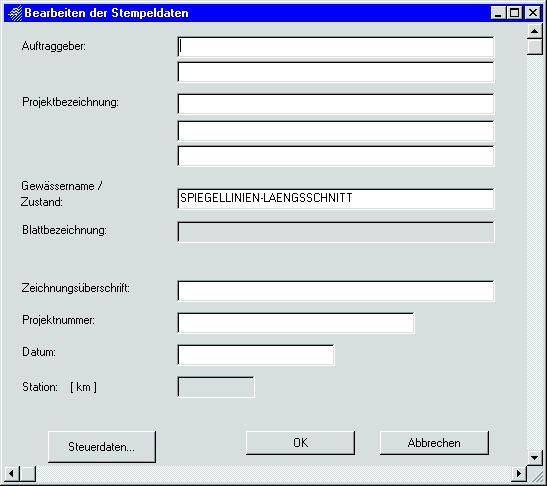
\includegraphics[width=0.9\textwidth]{PlottenStempeldaten}
   \caption{Eingabe der Stempeldaten}
   \label{Fortgeschrittene Abb PlottenStempeldaten}
\end{figure}

\"{U}ber die Schaltfl\"{a}che \schalter{Steuerdaten...} werden die Dialogmasken zur Festlegung Art und Weise der
Stationsbeschriftung aufgerufen (Abbildungen~\ref{Fortgeschrittene Abb Stationsbeschriftung_I} und \ref{Fortgeschrittene Abb Stationsbeschriftung_II}).

\subsubsection{Schriftfeld}
Die Darstellung im Schriftfeld beinhaltet die tabellarische Auflistung der berechneten oder eingegebenen Daten. Das
Schriftfeld besteht aus mindestens zwei Zeilen. Eine Zeile ist jeweils in einen Block f\"{u}r die Bezeichnung und einen f\"{u}r
die dazugeh\"{o}rigen Daten unterteilt. Der erste Datensatz der Profildatei (Gel\"{a}ndeh\"{o}he) wird dabei stets durch zwei
Schriftfeldzeilen, der Stationierungszeile und der Datenzeile, dargestellt. F\"{u}r alle weiteren Datens\"{a}tze ist die
M\"{o}glichkeit gegeben, Stations- und H\"{o}henwerte in dieselbe Schriftfeldzeile einzutragen. Dabei werden Stationswerte stets
links und H\"{o}henwerte stets rechts vom Bezugspunkt eingetragen.
\begin{figure}
   \centering
      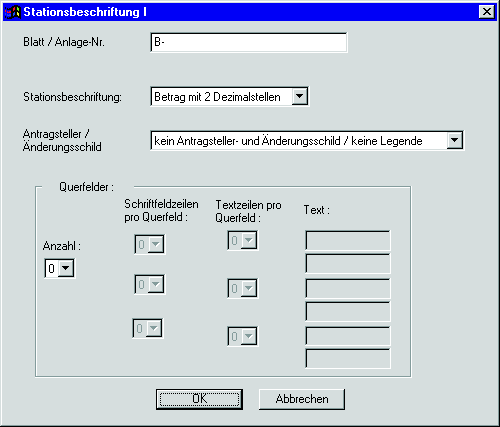
\includegraphics[width=0.75\textwidth]{PlottenStationsbeschriftung_I}
      \caption{Erstes Dialogfenster zur Stationsbeschriftung}
      \label{Fortgeschrittene Abb Stationsbeschriftung_I}
\end{figure}

\begin{figure}
    \centering
      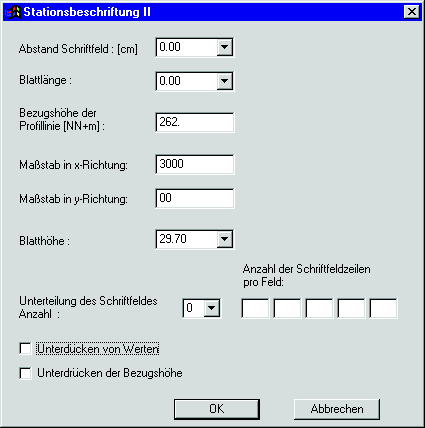
\includegraphics[width=0.75\textwidth]{PlottenStationsbeschriftung_II}
      \caption{Zweites Dialogfenster zur Stationsbeschriftung}
      \label{Fortgeschrittene Abb Stationsbeschriftung_II}
\end{figure}

\begin{sidewaysfigure}
   \centering
   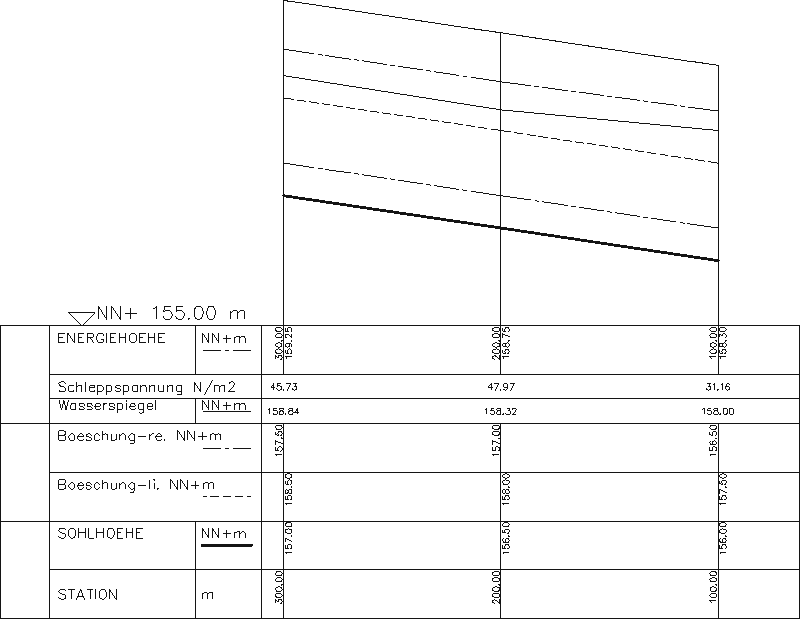
\includegraphics[width=0.9\textwidth]{Laengsschnittplott}
   \caption{L\"{a}ngsschnittplott mit verschiedenen Schriftfelddarstellungen}
   \label{Fortgeschrittene Abb Laengsschnittplott}
\end{sidewaysfigure}

Die Schaltfl\"{a}che \schalter{Steuerdaten} im Dialog \dialog{Bearbeiten der Stempeldaten} f\"{u}hrt sie in die Umgebung zur
Festlegung der Darstellungsform des Schriftfeldes. Mehreren Schriftfeldzeilen kann mit Hilfe von Querfeldern eine
Beschriftung voran gestellt werden. Neben der Anzahl der Querfelder, mu{\ss} dazu auch die Anzahl der Schriftfeldzeilen
angegeben werden, die das Querfeld verbinden soll. Jedem Querfeld k\"{o}nnen ein oder zwei Textzeilen zugeordnet werden.

Die Bezeichnung einer Schriftfeldzeile (d.h. eines Datensatzes) kann bis zu zwei Textzeilen lang sein. F\"{u}r eine schmale
Schriftfeldzeile wird der Text, wenn er aus zwei Textzeilen besteht, verkleinert. Manche Schriftfeldzeilen bestehen nur
aus Erl\"{a}uterungstext, andere haben in der Regel auch eine Ma{\ss}einheit. Daher kann dieses Feld weiter unterteilt werden. Auf
der linken Seite steht dann die Bezeichnung, auf der rechten Seite die Ma{\ss}einheit und der Linientyp, wenn die Werte
grafisch dargestellt werden. Damit ergeben sich folgende Darstellungsformen einer Schriftfeldzeile:
\begin{itemize}
   \item keine Schriftfeldzeile
   \item schmale Schriftfeldzeile ohne Unterteilung (vgl. Datensatz \afz{Schleppspannung} in
         Abbildung~\ref{Fortgeschrittene Abb Laengsschnittplott})
   \item schmale Schriftfeldzeile mit Unterteilung (vgl. Datensatz~\afz{Wasserspiegel} in
         Abbildung~\ref{Fortgeschrittene Abb Laengsschnittplott})
   \item breite Schriftfeldzeile ohne Unterteilung (vgl. Datens\"{a}tze~\afz{B\"{o}\-schung li.} und \afz{B\"{o}\-schung re.} in
         Abbildung~\ref{Fortgeschrittene Abb Laengsschnittplott}
   \item breite Schriftfeldzeile mit Unterteilung (vgl.
         Ab\-bil\-dung~\ref{Fortgeschrittene Abb Laengsschnittplott}, Datensatz~\afz{Sohlh\"{o}he})
\end{itemize}

Blattgr\"{o}{\ss}e, Ma{\ss}stab und Schriftfeldabstand zum Zeichnungsrand werden im Dialog \dialog{Stationsbeschriftung II}
festgelegt. Weiterhin ist die Bezugsh\"{o}he einzugeben, \"{u}ber der der Auftrag der Profile erfolgen soll. Eine Beschriftung der
Bezugsh\"{o}he kann mit Hilfe von \checkbox{Unterdr\"{u}cken der Bezugsh\"{o}he} unterbunden werden. Zus\"{a}tzlich zu dem Voranstellen
einer Beschriftung in einem Querfeld vor mehrere Schriftfeldzeilen kann die Zusammengeh\"{o}rigkeit von Daten auch durch
Rahmen kenntlich gemacht werden. Dazu ist im unteren Teil der Dialogmaske die Anzahl der Unterteilungen des Schriftfeldes
anzugeben. Maximal sind f\"{u}nf Unterteilungen m\"{o}glich. Jeder Unterteilung ist danach die gew\"{u}nschte Anzahl der
Schriftfeldzeilen zuzuordnen. Wird die Option \checkbox{Unterdr\"{u}cken von Werten} aktiviert, so werden nur die Daten
dargestellt, f\"{u}r deren Beschriftung ausreichend Platz vorhanden ist.
\begin{figure}[hbt]
   \centering
   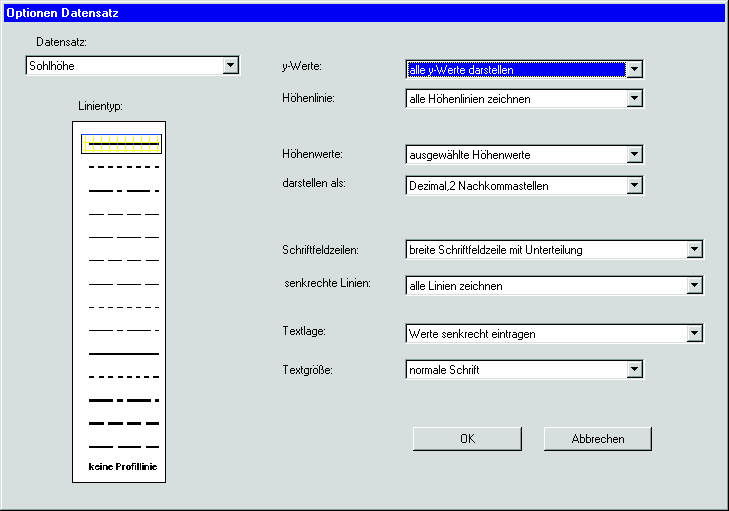
\includegraphics[width=1.0\textwidth]{PlottenOptionenDatensatz}
   \caption{Dialog zur Darstellung der Datens\"{a}tze}
   \label{Fortgeschrittene Abb OptionenDatensatz}
\end{figure}





\subsubsection{Darstellung der Daten}
Der letzte Dialog (Abbildung~\ref{Fortgeschrittene Abb OptionenDatensatz}) betrifft die Darstellung der einzelnen
Datens\"{a}tze auf der Zeichnung. Die Darstellung der Daten im Schriftfeld kann auf verschiedene Art und Weise erfolgen. Dies
betrifft sowohl das Zahlenformat, die Ausrichtung als auch die Datenmenge. Im Dialogfenster \dialog{Optionen Datensatz}
(Abbildung~\ref{Fortgeschrittene Abb OptionenDatensatz}) werden dazu zun\"{a}chst alle vorhandenen Datens\"{a}tze in einer Liste
links oben angezeigt. Durch Auswahl eines Datensatzes kann ihm das entsprechende Datenformat zugewiesen werden. Soll der
komplette Datensatz im Schriftfeld nicht dargestellt werden, so ist aus der Liste \feld{Schriftfeldzeilen} \afz{keine
Schriftfeldzeile} auszuw\"{a}hlen.

Unter dem Listenfeld mit den Datens\"{a}tzen finden Sie eine Auswahlm\"{o}glichkeit f\"{u}r das Darstellungsformat Ihrer Profillinien.
Die $y$- und $z$-Werte k\"{o}nnen jeweils alle, gar nicht oder als Auswahl dargestellt werden. Die Auswahl einzelner Werte
erfolgt ein einem gesonderten Dialog. In gleicher Weise l\"{a}{\ss}t sich auch die Darstellung der H\"{o}henlinien beeinflussen.

Darunter finden Sie das Listenfeld zur Darstellungsform der Schriftfeldzeilen. Der Text kann waagerecht und senkrecht in
verschiedenen Schriftgr\"{o}{\ss}en eingetragen werden.
\begin{quote}
   \begin{tabular}{ll}
      kleine Schrift:          &    $1,0\unit{mm}$ \\
      normale Schrift: \qquad  &    $2,0\unit{mm}$ \\
      Gro{\ss}e Schrift:           &    $3,0\unit{mm}$
   \end{tabular}
\end{quote}
Werden sowohl $y$- als auch $z$-Werte an einer Station angezeigt, so erfolgt die Darstellung der Daten \"{u}bereinander (vgl.
Abbildung~\ref{Fortgeschrittene Abb Laengsschnittplott} \afz{Energieh\"{o}he}). Es ist jedoch auch eine Ausgabe der $z$-Werte
auf der H\"{o}he der Station m\"{o}glich. Die Daten werden im Normalfall an senkrechten Linien im Schriftfeld ausgerichtet. Sie
lassen sich so einer exakten Position zuordnen. Besonders bei einer H\"{a}ufung von Daten in bestimmten Bereichen kann es
sinnvoll sein, nicht alle Linien darstellen zu lassen, da es hier u.U. zu einer \"{U}berschneidung in der Darstellung kommt.
Haben sie zur Darstellung der Linien im Datensatz \afz{Sohlh\"{o}he} bereits eine Auswahl getroffen, so kann diese Auswahl in
den anderen Datens\"{a}tzen \"{u}bernommen werden. Nach dem Best\"{a}tigen der Eingabe mit \schalter{OK} gelangen Sie zur\"{u}ck in das
Dialogfenster \dialog{Bearbeiten der Stempeldaten}.


\subsubsection{Plotten Konfiguration}
\wspwin{} wird mit einer Plotterkonfigurationsdatei geliefert. Die Konfigurationsdatei dient dazu, einzelnen Layern Stifte
unterschiedlicher Strichst\"{a}rke oder Farbe zuzuordnen. Dabei werden den einzelnen Layern (z.B. Gel\"{a}ndelinie, Text) die
Nummern der Stifte des Plotters zugewiesen. Die mitgelieferte Plotterkonfigurationsdatei \datei{plotter.cfg} ist auf einen
speziellen Farbplotter angepa{\ss}t, bei dem Sie unter dem Men\"{u} \menu{\marrow P\underline{l}otten \marrow D\underline{X}F
\marrow \underline{K}onfiguration} den einzelnen Layern verschiedene Farben (z.B. Sohlh\"{o}he blau) zuweisen k\"{o}nnen. Eine
\"{U}bersicht welche Linientypen in welchen Layern repr\"{a}sentiert werden, findet sich in Abbildung~\ref{Fortgeschrittene Abb
LinienLayer}.
\begin{figure}[hbt]
   \centering
   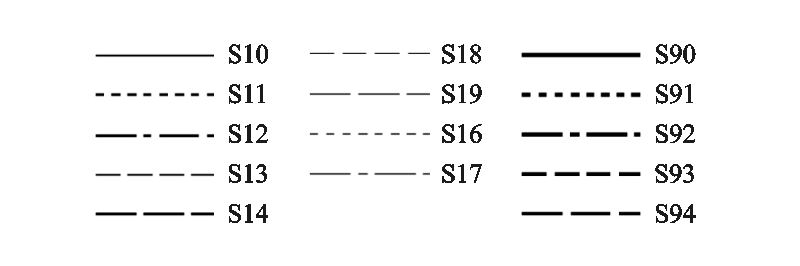
\includegraphics[width=0.7\textwidth]{LinienLayer}
   \caption{Linientypen und zugeordnete Layer}
   \label{Fortgeschrittene Abb LinienLayer}
\end{figure}


\subsection{CAD-Programm}

Zur Einsicht und zum Bearbeiten der erstellten \datei{*.dxf}-Dateien kann \"{u}ber diesen Men\"{u}punkt ein externes CAD-Programm
gestartet werden. Im Men\"{u} \menu{\marrow E\underline{x},0tras} sind dazu die entsprechenden Einstellungen gem\"{a}{\ss}
Abschnitt~\ref{Installation Subsec Verzeichnisse} vorzunehmen.
